\documentclass{article}
% preamble.tex
\usepackage{amsmath, amsthm, amssymb}
\usepackage{mathtools}
\usepackage{mathabx}
\usepackage{adjustbox}
\usepackage{graphicx}% Required for inserting images
\usepackage{tikz-cd} 
\usepackage{tikz}
\usepackage{comment}
\usetikzlibrary{calc, graphs, positioning, backgrounds, decorations.pathmorphing}
\usepackage{forest}
\usepackage{pgfplots, pgfplotstable}
\usepackage{indentfirst}
\pgfplotsset{compat=1.17}
\usepackage[a4paper,width=150mm,top=25mm,bottom=25mm]{geometry}
\usepackage{fancyhdr}
\pagestyle{fancy}
\usepackage{ifthen}
\usepackage{float}
\usepackage{subcaption}
\usepackage{xkeyval} % Load xkeyval first
\usepackage[colorlinks=true,linkcolor=blue]{hyperref} % Load hyperref with simplified options
\usepackage[dvipsnames]{xcolor}
\usepackage{tcolorbox}
\usepackage{wrapfig}
\usepackage[framemethod=tikz]{mdframed}
\usepackage{atbegshi}% http://ctan.org/pkg/atbegshi


\definecolor{block-gray}{gray}{0.95}
\newtcolorbox{examplesblock}[2][]{%
    grow to right by=-0mm,
    grow to left by=-0mm, 
    opacityback=0,
    frame hidden, boxrule=0pt,
    boxsep=0pt,
    breakable,
    enhanced jigsaw,
    borderline west={2pt}{0pt}{black},
    title={#2\par},
    colbacktitle={black},
    coltitle={black},
    fonttitle={\bfseries},
    attach title to upper={},
    #1,
}

\definecolor{}{gray}{0.95}
\newtcolorbox{codeblock}[2][]{%
    grow to right by=-0mm,
    grow to left by=-0mm, 
    opacityback=0,
    frame hidden, boxrule=0pt,
    boxsep=0pt,
    breakable,
    enhanced jigsaw,
    borderline west={2pt}{0pt}{black},
    title={#2\par},
    colbacktitle={black},
    coltitle={black},
    fonttitle={\large\bfseries},
    attach title to upper={},
}

\titleformat{\chapter}[display]   
{\normalfont\huge\bfseries}{\chaptertitlename\ \thechapter}{20pt}{\Huge}   
\titlespacing*{\chapter}{0pt}{-30pt}{40pt}

\newtheoremstyle{mystyle}%                % Name
  {1pt}%                                     % Space above
  {}%                                     % Space below
  {\normalfont}%                                     % Body font
  {}%                                     % Indent amount
  {\bfseries}%                            % Theorem head font
  {.}%                                    % Punctuation after theorem head
  { }%                                    % Space after theorem head, ' ', or \newline
  {\thmname{#1}\thmnumber{ #2}\thmnote{ (#3)}}%                                     % Theorem head spec (can be left empty, meaning `normal')

  \theoremstyle{mystyle}
\newtheorem*{remark}{Remark}

\NewDocumentCommand{\newframedtheorem}{O{}momo}{%
  \IfNoValueTF{#3}
   {%
    \IfNoValueTF{#5}
     {\newtheorem{#2}{#4}}
     {\newtheorem{#2}{#4}[#5]}%
    }
   {\newfratheorem{#2}[#3]{#4}}
  \tcolorboxenvironment{#2}{#1}%
}
\newmdtheoremenv{theorem}{Theorem}[section]


\newtheorem{corollary}{Corollary}[section]
\newmdtheoremenv{boxcor}{Corollary}[theorem]
\newtheorem{lemma}[theorem]{Lemma}
\newtheorem{prop}[section]{Proposition}
\newtheorem{definition}{Definition}[section] 
%\newtheorem{theorem}{Theorem}[section] 

\newmdtheoremenv{boxdef}{Definition}[section]
\newmdtheoremenv{boxlemma}{Lemma}[section]
\newmdtheoremenv{boxprop}{Proposition}[section]

\newcommand{\here}[2]{\tikz[remember picture]{\node[inner sep=0](#2){#1}}}

\newcommand{\N}{\ensuremath{\mathbb{N}}}
\newcommand{\R}{\ensuremath{\mathbb{R}}}
\newcommand{\Z}{\ensuremath{\mathbb{Z}}}
\newcommand{\Q}{\ensuremath{\mathbb{Q}}}
\newcommand{\C}{\ensuremath{\mathbb{C}}}
\newcommand{\PP}{\ensuremath{\mathbb{P}}}
\newcommand{\F}{\mathcal{F}}

\newcommand{\Real}{\operatorname{Re}}
\newcommand{\Img}{\operatorname{Im}}

\DeclareMathOperator{\spn}{span}
\DeclareMathOperator{\Id}{Id}
\DeclareMathOperator{\essup}{essup}
\DeclareMathOperator{\scrC}{\mathcal{C}}
\DeclareMathOperator{\scrM}{\mathcal{M}}
\DeclareMathOperator{\supp}{supp}
\DeclareMathOperator{\intr}{int}
\DeclareMathOperator{\conv}{conv}
\DeclareMathOperator{\diam}{diam}
\DeclareMathOperator{\ext}{Ext}
\DeclareMathOperator{\dist}{dist}


\newcommand{\inmath}[2]{$#1\in#2$}
\newcommand{\allin}[2]{for all $#1\in#2$}
\newcommand{\isthere}{there exists }

\newcommand{\vectsp}[1]{\mathbf{#1}}
\newcommand{\norm}[1]{\left\lVert#1\right\rVert}
\newcommand{\unitball}[1]{B_{#1}}
\newcommand{\intunitball}[1]{D_{#1}}
\newcommand{\unitsphere}[1]{S_{#1}}

\newcommand{\bigslant}[2]{{\raisebox{.2em}{$#1$}\left/\raisebox{-.2em}{$#2$}\right.}}
\newcommand{\bracket}[2]{\langle #1, #2\rangle}
 % Method of Enrico Gregorio ("egreg")
 % https://tex.stackexchange.com/a/22255/13492:
 \newcommand\restrict[2]{% make the whole thing an ordinary symbol
   \left.\kern-\nulldelimiterspace % automatically resize the bar with \right
   #1% the function
   \littletaller % pretend it's a little taller at normal size
   \right|_{#2}%
   }
 \newcommand{\littletaller}{\mathchoice{\vphantom{\big|}}{}{}{}}

 % Method of Heiko Oberdiek
 % https://tex.stackexchange.com/a/67233/13492
 \makeatletter
 \newcommand*{\scaleddelims}[3]{%
   \ensuremath{%
     \mathpalette{\@scaleddelims{#1}{#2}}{#3}%
   }%
 }   
 \newcommand*{\@scaleddelims}[4]{%
   % #1: left delimiter
   % #2: right delimiter
   % #3: \displaystyle, \textstyle, ...
   % #4: inner formula
   \begingroup
     #3%
     \sbox0{$\m@th#3\vphantom{A}#4$}%
     \setbox2\vbox{\hbox{$\m@th#3#1$}\kern\z@}%
     \setbox4\vbox{\hbox{$\m@th#3#2$}\kern\z@}%
     \setbox6\hbox{$#3\vcenter{}$}%
     \ifx\downharpoonleft#1\relax  
       \let\DelimLeft=L%
     \else\ifx\upharpoonleft#1%
       \let\DelimLeft=L%
     \else\ifx\downharpoonright#1%
       \let\DelimLeft=R%
     \else\ifx\upharpoonright#1%
       \let\DelimLeft=R%
     \fi\fi\fi\fi
     \ifx\downharpoonleft#2\relax
       \let\DelimRight=L%
     \else\ifx\upharpoonleft#2\relax
       \let\DelimRight=L%
     \else\ifx\downharpoonright#2\relax
       \let\DelimRight=R%
     \else\ifx\upharpoonright#2\relax
       \let\DelimRight=R%
     \fi\fi\fi\fi
     \ifx\DelimLeft L%
       \wd2=.6\wd2
     \fi
     \ifx\DelimRight L%
       \wd4=.6\wd4
     \fi
     \ifx\DelimLeft R%
       \sbox2{\kern-.4\wd2\box2}%
     \fi
     \ifx\DelimRight R%
       \sbox4{\kern-.4\wd4\box4}%
     \fi
     \dimen0=\ht0 %
     \advance\dimen0 by -\ht6 %
     \dimen2=\dp0 %
     \advance\dimen2 by \ht6 %
     \ifdim\dimen2>\dimen0 %  
       \dimen0=\dimen2 %
     \else
       \dimen0=\dimen0 %
     \fi
     \dimen2=\ht6 %
     \advance\dimen2 by -\dimen0 %
     \dimen0=2\dimen0 %
     \def\DelimCorr{%  
       \mskip.5\thinmuskip
       \nonscript\mskip.5\thinmuskip
     }%
     \mathopen{%
       \ifx\DelimLeft R\DelimCorr\fi
       \raisebox{\dimen2}{\resizebox{!}{\dimen0}{\box2}}%
       \ifx\DelimLeft L\DelimCorr\fi
     }%
     \begingroup
       #3#4%
     \endgroup
     \mathclose{%
       \ifx\DelimRight R\DelimCorr\fi
       \raisebox{\dimen2}{\resizebox{!}{\dimen0}{\box4}}%
       \ifx\DelimRight L\DelimCorr\fi
     }%
   \endgroup
 }\makeatother
 %

 \newcommand{\restr}[2]{#1\scaleddelims{\kern-0.5\nulldelimiterspace\upharpoonright}{\vphantom{.}}{_{#2}}}
\newcommand{\diff}{\ensuremath{\operatorname{d}\!}}

  % Include the preamble from an external file
\usepackage{algorithm}
\usepackage{algpseudocode}
\usepackage{enumitem}% http://ctan.org/pkg/enumitem

%\AtBeginDocument{\AtBeginShipoutNext{\AtBeginShipoutDiscard}\addtocounter{page}{-1}}
\fancyhead{}
\fancyhead[L]{\text{Imperial UROP 2023}}
\fancyhead[R]{\text{Pantelis Tassopoulos}}

\title{\Huge Imperial College Summer Research \\ 
\huge Under the supervision of Professor Greg Pavliotis}
\author{\Large Pantelis Tassopoulos}
\date{\Large Summer 2023}

\begin{document}


\maketitle
\newpage

\tableofcontents 
\newpage 

\section{Overview}

\subsection{Objectives}

\begin{itemize}
	\item	To examine the existing literature on recent developments in the context of theoretical machine learning that integrate tools from statistical physics and probability theory, i.e., the theory of interacting particle systems.
	\item 	To analyse the approximation quality and trainability of neural networks using algorithms, such as Stochastic Gradient Descent (SGD), informed by such ideas on toy models and examples with real life examples such as the MNIST digit classification dataset.
	\item 	To perform numerical experiments by training neural networks under various circumstances, thereby graining practical insights. 
	\item 	To try and extend results from the literature by attempting to provide theoretical guarantees for accuracy and robustness of machine learning algorithms other than SGD or new insights from numerical simulations. 

\end{itemize}

\subsection{Outcomes}

This Summer Project (UROP) gave me a better insight into cutting-edge research in theoretical machine learning and mathematical optimisation.\\ 

I reviewed the requisite background material in mathematics from reference material, including textbooks and relevant papers. For instance, I read up on topics in probability, namely, martingale inequalities (Doob's and Hoeffman's inequalities in the book of Bremaud entitled 'Probability Theory and Stochastic Processes' \cite{bremaud2020probability}) that Mei et al. in their 2018 paper entitled 'A mean-field view of the landscape of two-layer neural networks' used in proofs of convergence of the SGD dynamics to the evolution of a Partial Differential Equation (PDE) as the hidden layer had an ever-increasing number of nodes, which enabled to perform novel theoretical analyses and provide theoretical guarantees of convergence.\\

I did some additional reading to supplement my understanding of the 2019 papers by Spiliopoulos and Sirgiano entitled 'Mean Field Analysis of Neural Networks: A Law of Large Numbers' and its companion paper \cite{sirignano2019meanfieldanalysisclt}, \cite{sirignano2019meanfieldanalysislln} . I read part of the book entitled 'Markov Processes: Characterisation and Convergence' by Stewart N. Ethier Thomas G. Kurtz \cite{ethier2009markov}, specifically the chapter on weak convergence of probability measures with values on the Skorokhod space $\mathcal{D}_{E[0, \infty)}$, which was necessary for understating the author's arguments on propagation of chaos and analogous convergence arguments. \\

Another crucial component of the project was the emphasis on numerical experiments. They allowed me to demonstrate the validity of theoretical findings and strengthen the case for the arguments presented. Numerical simulations involved training neural networks using existing algorithms from the literature and using insights gained to develop new algorithms. \\

For instance, regarding the above papers by Spiliopoulos, to supplement my understanding and empirically demonstrate claims made in the above paper, I performed numerical simulations by training a family of single-layer neural networks that achieved single-digit classification on the MNIST data set (used for digit classification and is a well-known benchmark for testing models). Upon expanding their hidden layer and training them, I plotted histograms of the distribution parameters which, for sufficiently many hidden nodes, the distribution of node values seemed to stabilise around a fixed bimodal distribution, which is also what the authors reported (while they did not specify the exact nature of the neural network they trained). \\

The project's theme shifted from analysing plain SGD towards understanding the wildly non-convex landscape of the underlying objective/loss function one typically encounters in machine learning applications.\\

In this direction, I demonstrated, among other observations, which can be found on my GitHub page \cite{Tassopoulos_Imperial_Summer_Research_2023} using numerical simulations that Nesterov accelerated gradient descent escaped a 'bad minimum', where SGD got stuck in a loss function that was constructed in \cite{Mei_2018}. \\

This motivated me to generalise further insights gained by examining the dynamics of SGD to momentum-based algorithms, including Nesterov's accelerated Gradient Descent. \\

At that time, I read the 2017 paper by Chaudhari et al. entitled 'Deep Relaxation: partial differential equations for optimising deep neural networks' \cite{Chaudhari2017DeepRP}. They introduced various approaches centred around 'regularising' the loss function. I incorporated both momentum-based methods (including 'restarting' the momentum if the gradient in the change in position was in the direction of the gradient-maximal increase, as was introduced in the 2012 Candes et al. paper entitled 'Adaptive Restart for Accelerated Gradient Schemes' \cite{odonoghue2012adaptiverestartacceleratedgradient}) and regularising the potential (by leveraging the analytical properties of solutions to the Hamilton-Jacobi-Bellman equation) as suggested above to create an algorithm that attempted to escape bad minima.\\

I also revisited the 2023 paper by Andrew Stuart et al. entitled 'Gradient Flows for Sampling: Mean-Field Models, Gaussian, Approximations and Affine Invariance'\cite{chen2023gradientflowssamplingmeanfield} initially suggested by my supervisor to produce another algorithm based on theoretical insights gained from the paper. \\

Furthermore, I read the paper coauthored by my supervisor entitled 'The sharp, the flat and the shallow: Can weakly interacting agents learn to escape bad minima?' \cite{kantas2019sharpflatshallowweakly} I was also led to study the analysis of multiscale algorithms in the literature, e.g. in the Weinan et al. (2005) paper \cite{weinan2005multiscalesde} on the analysis of multiscale methods for SDEs. The authors devised an algorithm that escaped bad minima in a toy example they introduced in the paper. \\

As suggested by my supervisor, I implemented the above algorithms by performing descent on a loss that was a Muller-Brown potential (the canonical example of a potential surface in theoretical chemistry). My instance had a narrow global minimum; SGD would perform poorly and tend to converge to two local minima, of which there were two in a relatively confined domain. For each algorithm mentioned above, I performed random initialisations, ran the algorithms for a fixed number of steps and recorded the final 'losses'. One notable observation is that the implementation of the algorithm in my supervisor’s paper performed noticeably better than the rest, including plain SGD.\\

This research experience presented an excellent opportunity for me to go beyond the scope of material covered in class and explore developments in the literature in a structured and rigorous manner. \\

Please note all the code referenced herein can be found on my personal GitHub page \cite{Tassopoulos_Imperial_Summer_Research_2023} . \\

\newpage
\section{Mean Field Limits of Neural Networks}\label{sec: mean field neural net}

\subsection{Background theory}\label{sec: neural net single layer}

The process of a neural network 'learning' from data requires solving a complex optimisation problem with millions of variables. This is done by stochastic gradient descent (SGD) algorithms. One can study the case of two-layer networks and derive a compact description of the SGD dynamics in terms of a limiting partial differential equation. This a major insight in \cite{Mei_2018}, where they authors also suggest with their findings that SGD dynamics do not become more complex when the network size increases.\\ 

Now, more formally, one typically encounters, in the context of supervised learning the following: 
\begin{itemize}
	\item Observed data points $ (x_{i},y_{i})_{i\in \N}\subseteq \R^{d}\times \R$, where they are modelled as being independent and indentically distributed (iid).
	\item The $ x\in \R^{d}$ are called \underline{feature vectors} and the $ y\in \R$ the \underline{labels}.
	\item The neural network essentially is a function that depends on some hidden parameters and the feature vector. In the case of a two-layer neural network, the dependence is modelled by: 
		\begin{equation}\label{eq: neural net def}
			\begin{array}{cc}
			\hat{y}:\R^{d}\times \R^{ND}\to \R   \\
			(x;\mathbf{\theta})\mapsto \frac{1}{N}\displaystyle\sum^{N}_{i=1}\sigma_{*}(x;\mathbf{\theta}_{i})     
	     \end{array}
     \end{equation}
		where $ N$ is the number of hidden units (neurons), $ \sigma_{*}:\R^{d}\times\R^{D}\to \R$ an activation function and $\mathbf{\theta} = (\mathbf{\theta})_{i\leq N}$, $\mathbf{\theta}_{i}\in \R^{D}$ are parameters, often $\mathbf{\theta}_{i} = (a_{i}, b_{i}, w_{i})$ for real $ a_{i}, b_{i}, w_{i}$ and $ \sigma_{*}(x;\mathbf{\theta}_{i})=a_{i}\sigma(\bracket{x}{w_{i}}+b_{i})$ for some function $ \sigma:\R\to \R$ (see figure \ref{fig: two layer neural net}).
\end{itemize}


\begin{figure}[H]
    \centering
    \begin{tikzpicture}[scale = 1.3, x=2cm, y=1.5cm, thick, every node/.style={scale=1}]

% Input node (smaller size)
\node[circle, draw, minimum size=0.7cm] (I) at (0, 0) {$\mathbf{x}$};

% Hidden nodes with labels on both sides (left and right)
\node[left=0cm of I] {};

\node[circle, draw, minimum size=0.7cm] (H1) at (1, 1.2) {};
\node[right=0cm of H1] {\scriptsize $\sigma_*(\mathbf{x};\mathbf{\theta}_1)$};  % Equation on the right with smaller size
\node[left=0.2cm of H1] {$\mathbf{\theta}_1$};        % Label on the left

\node[circle, draw, minimum size=0.7cm] (H2) at (1, 0.4) {};
\node[right=0cm of H2] {\scriptsize $\sigma_*(\mathbf{x};\mathbf{\theta}_2)$};  % Equation on the right with smaller size
\node[left=0.2cm of H2] {$\mathbf{\theta}_2$};        % Label on the left

\node at (1, -0.4) {$\vdots$};             % Ellipsis between nodes

\node[circle, draw, minimum size=0.7cm] (H3) at (1, -1.2) {};
\node[right=0cm of H3] {\scriptsize $\sigma_*(\mathbf{x};\mathbf{\theta}_N)$};  % Equation on the right with smaller size
\node[left=0.2cm of H3] {$\mathbf{\theta}_N$};        % Label on the left

% Output node (smaller size)
\node[circle, draw, minimum size=0.7cm] (O) at (2, 0) {$\hat{y}$};

% Connections
\draw[->] (I) -- (H1);
\draw[->] (I) -- (H2);
\draw[->] (I) -- (H3);

\draw[->] (H1) -- (O);
\draw[->] (H2) -- (O);
\draw[->] (H3) -- (O);

\end{tikzpicture}
    \caption{ Illustration of a two layer neural network.}
    \label{fig: two layer neural net}
\end{figure}


Naturally, one wants to chose parameters $\mathbf{\theta}$ so as to \underline{minimise} the risk function 
\begin{equation}\label{eq: risk}
	R_{N}(x;\mathbf{\theta}) =\mathbb{E}[\ell(y, \hat{y}(x;\mathbf{\theta}))]
\end{equation}

for a loss function $ \ell:\R\times \R \to \R$, typically and in our case the square loss $ \ell(y-\hat{y})  = (y-\hat{y})^{2}$. This is achieved in practice by stochastic gradient descent summarised below:


\newpage
\begin{codeblock}{Stochastic Gradient Descent (SGD)}\label{alg: SGD}
\begin{algorithmic}
\State Initialise the parameters $(\mathbf{\theta}_{i})_{i\leq \N} \sim \rho_{0}$, that is according to some initial distribution $ \rho_{0}$.
\While{loss is greater than tolerance}
\State Generate iid sample $ (x, y)\sim \PP$
\For {$1 \leq i \leq N $} 
\State $\mathbf{\theta}_{i}\gets\mathbf{\theta}_{i}+2s\cdot (y-\hat{y}(x;\mathbf{\theta}))\cdot \nabla_{\mathbf{\theta}_{i}}\sigma_{*}(x;\mathbf{\theta}_i)$ \Comment{square loss is used}
\State Update learning rate $ s$
\EndFor
\EndWhile
\end{algorithmic}

\end{codeblock}

Observe that we have the alternative characterisation of the loss
\begin{equation}\label{eq: loss expanded}
	R_{N}(\mathbf{\theta}) = R_{\#}+ \frac{2}{N}\displaystyle\sum^{N}_{i=1}V(\mathbf{\theta}_{i})+\frac{1}{N^{2}}\displaystyle\sum^{N}_{i,j=1}U(\mathbf{\theta}_{i},\mathbf{\theta}_{j}).
\end{equation} 
where $ V(x; \mathbf{\theta}) = -\mathbb{E}[y\cdot \sigma_(x: \mathbf{\theta})]$, $ U( \mathbf{\theta}_{1}, \mathbf{\theta}_{2}) =\mathbb{E}[\sigma_(x; \mathbf{\theta}_{1})\cdot \sigma_*(x; \mathbf{\theta}_{2})]$ and $ R_{\#}=\mathbb{E}[y^{2}]$ is the risk of the trivial predictor $ \hat{y} = 0$.\\ 

Notice that the collection of weights $  \mathbf{\theta}\in \R^{ND}$ induces a probability measure on $ \R^{ND}$, namely its \textit{empirical measure}:

\begin{equation}\label{eq: empirical measure}
	\hat{\rho}^{(N)} = \frac{1}{N}\displaystyle\sum^{N}_{i=1}\delta_{ \mathbf{\theta}_{i}} 
\end{equation}

Consider the function on the space of probability measures on $ \R^{D}$, $  \mathcal{P}(\R^{D})$:
\[
\begin{array}{cc}
    R: \mathcal{P}(\R^{D})\to \R \\ 
    \rho \mapsto R_{\#}+ 2 \displaystyle\int V( \mathbf{\theta}) \rho( \diff \mathbf{\theta}) + \displaystyle \int\int U( \mathbf{\theta}_{1}, \mathbf{\theta}_{2}) \rho( \diff \mathbf{\theta}_{1}) \rho( \diff \mathbf{\theta}_{2})   
\end{array}
\]
Observe we can thus express $ R_{N}(\mathbb{\theta}) = R(\hat{\rho}^{(N)})$. Now, performing the SGD algorithm \ref{alg: SGD} for $ k$ steps say (with step size $ s_k = \epsilon\cdot \xi(k \epsilon)$ for some $ \epsilon >0$ and $ \xi: \R_{\geqq 0}\to \R_{\geqq 0}$ sufficiently regular-see \ref{list: reg assumptions}), we obtain the parameters $  (\mathbf{\theta}^{k}_{i\leq N})$ and their respective empirical measures $ \hat{\rho}^{(N)}_k$. In \cite{Mei_2018}, Theorem \ref{thm: mean field nguyen} here, it is shown that for all $ t\geqq 0$, as $ N\to \infty$ and $ \epsilon \to 0$ in an appropriate way, the empirical measures $ \hat{\rho}^{(N)}_{t/\epsilon}$ converge in the weak sense to some probability measure $ \rho_t$ whose dynamics are governed by the following PDE, which is referred to as \emph{distributional dynamics} (DD) in \cite{Mei_2018}
\begin{equation}
	\begin{array}{ll}
\partial_t \rho_t & =2\xi(t)\, \nabla_{ \mathbf{\theta}}\cdot \Big(\rho_t \nabla_{ \mathbf{\theta}}\Psi( \mathbf{\theta};\rho_t)\Big)\, ,\label{eq:GeneralPDE}\\
\Psi( \mathbf{\theta};\rho) & \equiv V( \mathbf{ \theta})+\int U( \mathbf{\theta}, \mathbf{\theta}')\, \rho(\diff  \mathbf{\theta}') .
\end{array}
\end{equation}

(Note that $\nabla_{ \mathbf{\theta}}\cdot \mathbf{v}( \mathbf{\theta})$ denotes the divergence of the vector field $ \mathbf{v}( \mathbf{\theta})$). This should  be interpreted as an evolution equation in $ \mathcal{P}(\R^D)$.\\

There is rich mathematical literature on the PDE \ref{eq:GeneralPDE} which was
motivated by the study of interacting particle systems in mathematical physics (see the references in \cite{Mei_2018}). The authors in \cite{Mei_2018} use this to observe that \ref{eq:GeneralPDE} can be viewed as a gradient flow for the cost function $R(\rho)$ in the space 
$( \mathcal{P}(\R^D),W_2)$, of probability measures on $\R^D$
endowed with the Wasserstein metric.\\

\begin{examplesblock}{Aside:}\label{aside: wasserstein flow}
Regarding Wasserstein flows, I looked through the paper by Y. Chen , et al. \cite{chen2023gradientflowssamplingmeanfield} on Gradient Flows for Sampling and noted down some key insights from their paperIn brief, they study the problem of sampling a probability distribution with an unknown normalization constant, which is a fundamental problem in computational science and engineering. They recast it as an optimisation problem on the space of probability measures, using gradient flows. 
\begin{enumerate}[(a)]
    
	\item 	Given a gradient flow that one has constructed wrt a posterior distribution that one wants to sample from without having an explicit normalization, one can formulate a gradient flow and a system of particles with SDE of the MCKean Vlasov type with FK equation the gradient flow (i.e. the evolution equation of the density). 
	\item 	By making the gradient flow ‘invariant’ under affine reparameterizations (through preconditioning or by suitable choice of metric or energy functional on $\mathcal{P}(\R^d))$, one hope to improve performance of algorithms in the case of highly anisotripic posteriors, if there is an affine transformation that reduces the anisotropic nature of said posterior.
\end{enumerate}
\end{examplesblock}



Recall that Wasserstein distance is defined as
\begin{equation}\label{eq:Wasserstein_dual}
W_2(\rho_1,\rho_2)  = \Big(\inf_{\gamma\in \mathcal{C}(\rho_1,\rho_2)}  \int \| \mathbf{\theta}_1- \mathbf{\theta}_2 \|_2^2 \gamma( \diff  \mathbf{\theta}_1, \diff \mathbf{\theta}_2) \,\Big)^{1/2}. 
\end{equation}

In order to establish that these PDEs indeed describe the limit of the SGD dynamics, we make the following assumptions.
%
\begin{itemize}\label{list: reg assumptions}
%
	\item[{\sf A1.}] $t\mapsto \xi(t)$ is bounded Lipschitz: $\|\xi\|_{\infty}, \|\xi\|_{\text{Lip}}\leq K_1$, with $\int_0^{\infty}\xi(t) \diff  t=\infty$.
%
\item[{\sf A2.}] The activation function $( \mathbf{x}, \mathbf{\theta})\mapsto \sigma_*( \mathbf{x}; \mathbf{ \theta})$ is bounded, with sub-Gaussian gradient: $\|\sigma_*\|_{\infty}\leq  K_2$, $\|\nabla_{ \mathbf{ \theta}}
\sigma_*( \mathbf{X}; \mathbf{\theta})\|_{\psi_2}\leq K_2$. Labels are bounded $|y_k|\leq K_2$.
%
\item[{\sf A3.}] The gradients $\mathbf{\theta}\mapsto \nabla V( \mathbf{\theta})$, $(\mathbf{\theta}_1,\mathbf{\theta}_2)\mapsto \nabla_{\mathbf{\theta}_1}U(\mathbf{\theta}_1,\mathbf{\theta}_2)$  are bounded, Lipschitz continuous 
(namely $\| \nabla_{\mathbf{\theta}}V(\mathbf{\theta}) \|_2$, $\|\nabla_{\mathbf{\theta}_1}U(\mathbf{\theta}_1,\mathbf{\theta}_2)\|_2\leq K_3$, $\|\nabla_{\mathbf{\theta}}V(\mathbf{\theta})-\nabla_{\mathbf{\theta}}V(\mathbf{\theta}')\|_2\leq K_3 \|\mathbf{\theta}-\mathbf{\theta}'\|_2$, $\|\nabla_{\mathbf{\theta}_1}U(\mathbf{\theta}_1,\mathbf{\theta}_2)-\nabla_{\mathbf{\theta}_1}U(\mathbf{\theta}'_1,\mathbf{\theta}_2')\|_2\leq K_3 \|(\mathbf{\theta}_1,\mathbf{\theta}_2)-
(\mathbf{\theta}_1',\mathbf{\theta}_2')\|_2$).
%
\end{itemize}

\begin{theorem}[PM. Nguyen et al. (2018)]\label{thm: mean field nguyen}
Assume that conditions {\sf A1}, {\sf A2}, {\sf A3} hold.
For $\rho_0\in\mathcal{P}(\R^D)$, consider SGD with initialization $(\mathbf{theta}^0_i)_{i\leq N}\sim_{iid}\rho_0$ and step size $s_k = \epsilon \xi(k \epsilon)$. For $t\geq 0$, let $\rho_t$ be the solution of PDE \ref{eq:GeneralPDE}.
Then, for any fixed $t \geq 0$,  $\hat{\rho}^{(N)}_{\lfloor t / \epsilon \rfloor} \Rightarrow \rho_{t}$ almost surely along any sequence $(N,\epsilon = \epsilon_N)$ such that $N \to \infty$, $\epsilon_N \to 0$, $N/\log (N/\epsilon_N) \to\infty$ and $\epsilon_N \log(N / \epsilon_N)\to 0$.
Further, there exists a constant $C$  (depending uniquely on the parameters $K_i$ of conditions {\sf A1}-{\sf A3}) such that,
for any $f:\R^D\times \R\to\R$, with $\|f\|_{\infty}, \|f\|_{\text{Lip}}\leq 1$, $\epsilon\leq 1$,
%
\begin{align}\label{eq: big theorem nguyen}
%
&\sup_{k \in  [0, T/\epsilon] \cap \N}\Big|\frac{1}{N}\sum_{i=1}^Nf(\mathbf{\theta}^{k}_i)- \int\!
  f(\mathbf{\theta})  \rho_{k\epsilon}(\diff \mathbf{\theta}) \Big| \leq Ce^{CT}\,\text{Err}_{N,D}(z)\, ,\nonumber\\
&\sup_{k \in  [0, T/\epsilon] \cap \N}\big|R_{N}(\mathbf{\theta}^{k})-R(\rho_{k\epsilon})\big| \leq Ce^{CT}\,\text{Err}_{N,D}(z)\, ,
%
\end{align} 
%
with probability $1- e^{-z^2}$ where $\text{Err}_{N,D}(z)$ is given by
\begin{equation}
	\sqrt{1/N\lor \epsilon}\cdot \left[ \sqrt{D + \log N/\epsilon}+z \right]
\end{equation}

\end{theorem}


\begin{theorem}[Doob's martingale inequality]\label{thm: Doob}
	Let $ (\F_{t})_{t\geq 0}$ be a filtration on the probability space $ (\Omega, \F, \PP)$ and $ (M_{t})_{t\geq 0}$ be a continuous martinagle adapted to the filtration $ (\F_{t})_{t\geq 0}$. Let $ p\geq 1$ and $ T>0$. If $\mathbb{E}[|M_{T}|^{p}]<\infty$ and $ \lambda > 0$, then 
	\begin{equation}
		\PP\left(\displaystyle\sup_{t\in [0,T]}|M_{t}|\geq \lambda\right)\leq \frac{\mathbb{E}[|M_{T}|^{p}]}{\lambda^{p}}
	\end{equation}
	
\end{theorem}

\begin{boxlemma}[Hoeffding's Lemma]\label{lemma: Hoeffding}
Let $ (M_{n})_{n\in\N}$ be a martingale adapted to the filtration $ (\F_{n})_{n\in\N}$ such that for some sequence $ c_{1}, c_{2},\cdots$ of real numbers 
\begin{equation}
	\PP(|M_{n}-M_{n-1}|\leq c_{n}) = 1 \quad \text{for all } n\in N.
\end{equation}
Then for all $ x\geq 0$ and all $ n\geq 1$,
\begin{equation}
    \PP(|M_{n}-M_{n-1}|\geq x)\leq 2 \exp \left( -\frac{1}{2}x^{2}\Big/\displaystyle\sum^{n}_{i=1}c_{i}^{2}  \right)
\end{equation}


\end{boxlemma}


\begin{proof}{(Rough Sketch)}
	The conditions {\sf A1} and {\sf A3} guarantee the existence and uniqueness of solutions to the PDE \ref{eq:GeneralPDE}, interpereted in the weak sense. The discrete SGD dynamics $ (\mathbf{\theta}_{i}^{k})_{i\leq N }$ appxorimate the continuous time dynamics. Then the proof becomes technical and the aim is to control error terms incurred when comparing the deviation of the discrete and continuous dynamics in probability.\\ 

    Notice we can also re-express \ref{eq: big theorem nguyen} in terms of the empirical measure to deduce for all function $ f$ with $ \norm{f}_{\text{Lip}}\leq 1$, $ \pi \in \mathcal{C}(\hat{\rho}^{N}_{k}, \rho_{k\epsilon})$ and $ k\in [0,T/\epsilon]$

\begin{equation}
	\begin{array}{ll}
	\Big|\displaystyle\int f(\theta)\hat{\rho}^{N}_{k}(\diff \theta)- \int\!
	f(\mathbf{\theta})  \rho_{k\epsilon}(\diff \mathbf{\theta}) \Big| &\leq  \displaystyle\int |f(\theta)-f(\phi)|\pi(\diff \theta, \diff \phi)\\ 
									  &\leq \displaystyle\int \norm{\theta-\phi}_{2}\pi(\diff \theta, \diff \phi)\leq W_{2}(\hat{\rho}^{N}_{k}, \rho_{k\epsilon}) 

\end{array}
\end{equation}
using Cauchy-Schwarz and taking the infimum over such couplings. Hence we obtain the bound 
\begin{equation}
    \sup_{k \in  [0, T/\epsilon] \cap \N}\Big|\displaystyle\int f(\theta)\hat{\rho}^{N}_{k}(\diff \theta)- \int\!
	f(\mathbf{\theta})  \rho_{k\epsilon}(\diff \mathbf{\theta}) \Big|\leq  \sup_{k \in  [0, T/\epsilon] \cap \N} W_{2}(\hat{\rho}^{N}_{k}, \rho_{k\epsilon}) 
\end{equation}
This estimate helps one get a sense of the terms that need to be controlled in the proof of the theorem.\\

	Moreover, the sub-gaussianity and Lipscitz continuity feature prominently and the tools used to achieve bounds on the the probabilities are mainly Doob's maximal inequality \ref{thm: Doob} and Hoefdding's lemma \ref{lemma: Hoeffding}. 
\end{proof}

The PDE formulation leads to several insights and simplifications. One can exploit symmetries in the data distribution $ \PP$ for instance. If $ \PP$ has rotational symmetry, then one can look for solutions to the PDE problem that share such rotational symmetry, thereby reducing the dimensionality of the problem which facilitates theoretical and numerical analysis. This is manifest in the case of two isotropic Gaussians considered later. Such symmetry cannot be achieved when considering the discrete dynamics since no set of poitns $ \mathbf{\theta}_{1}, \cdots, \mathbf{\theta}_{N}\in \R^{d}$ is invariant under rotations (excluding trivial cases).


\subsection{Centred Isotropic Gaussians}

The authors in \cite{Mei_2018} were interested in numerically testing their PDE framework on the classification problem of Gaussians with the same mean. That is, assume the joint law $ \PP$ of $(\mathbf{x}, y) $ to be:
\begin{equation}
\begin{array}{cc}
& \text{with probability}  1/2: y = +1, \mathbf{x}\sim N(0, (1+\Delta)^{2}\cdot\Id_{d})\\
& \text{with probability} 1/2: y = -1, \mathbf{x}\sim N(0, (1-\Delta)^{2}\cdot\Id_{d})
\end{array}
\end{equation}

For the activation function set $ \sigma( \mathbf{x}; \mathbf{\theta}) = \sigma(\bracket{w}{ \mathbf{x}})$ where $ \sigma$ is a simple piewewise linear activation function.\\

To try and reproduce the findings in \cite{Mei_2018},I implemented the SGD and the asymptotic PDE for the isotropic Gaussian case (SGD for isotropic gaussians with $10^7$ iterations) with $(w_i^0 )_{i\leq\N} \sim_{iid} \rho_0$, where $\rho_0$ is spherically symmetric. More specifically, I ran a monte carlo simulation of the discrete SGD dynamics and recorded the distance of the particles (hidden parameters $ \mathbf{\theta}$) after a set amount of iterations and aggreagated them, producing figure \ref{fig: SGD histogram isotropic Gaussians}. It compares nicely with the last subplot in \ref{fig: Nguyen 2018 isotropic Gaussian simulation}. 

\begin{figure}[H]
\begin{subfigure}{0.5\textwidth}
  \centering
  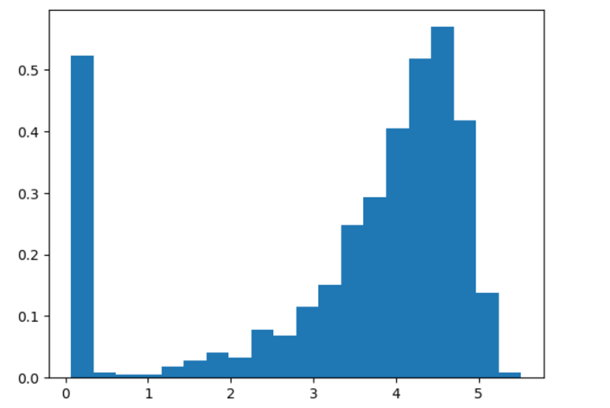
\includegraphics[width=0.8\linewidth]{ images/Nguyen2018-SGD-1.png}
  \caption{fig: SGD histogram for isotropic Gaussians\\ with $ 10^{7}$ iterations.}
  \label{fig: SGD histogram isotropic Gaussians}
\end{subfigure}%
\begin{subfigure}{0.5\textwidth}
  \centering
  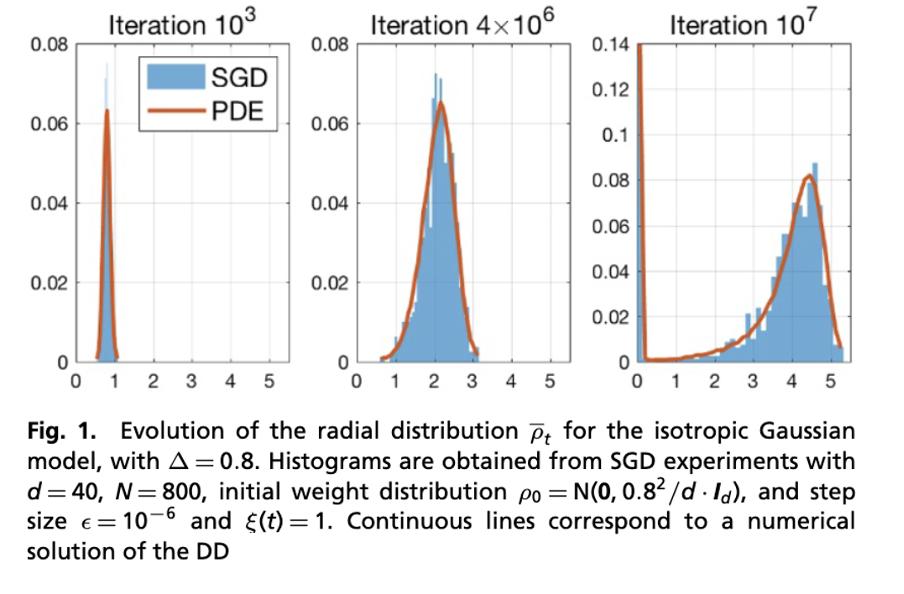
\includegraphics[width=0.8\linewidth]{images/Nguyen2018-paper-numerical-validation-iso-gauss.png}
  \caption{Corresponding simulation in the paper\\ by Nguyen et al.}
  \label{fig: Nguyen 2018 isotropic Gaussian simulation}
\end{subfigure}
\caption{Isotropic Gaussian SGD simulation.}
\label{fig:  isotropic gaussians SGD}
\end{figure}


Upon suggestion of my supervisor, I studied the possible non-uniqueness of stationary states for the mean field PDE that is derived in the paper by Mei et al.’ and its connection to the fact that SGD does not always converge to a near global optimum. There they introduce a non-monotone activation function
\begin{equation}
	\sigma_*( \mathbf{x}; \mathbf{\theta})= \sigma(\bracket{w}{x}), 
\end{equation}
where $\sigma(t) = −2.5 for t \leq 0, σ(t) = 7.5$ for $t \geq 1.5$, and $\sigma(t)$ linearly
interpolates from $(0, −2.5)$ to $(0.5, −4)$, and from $(0.5, −4)$ to $(1.5, 7.5)$, see figure \ref{fig: non-monotone activation fn}.

\begin{figure}[H]
    \centering
    \includesvg[width=0.6\linewidth]{images/non-monotone-activation.svg}
    \caption{Non-monotone activation function $\sigma$.}
    \label{fig: non-monotone activation fn}
\end{figure}

\noindent Depending on the initialization,
\begin{equation}
(w^{0}_{i})_{i\leq N}\sim_{iid} N(0, \kappa^{2}/d\Id_{d})
\end{equation}
with $ \kappas = 0.4, 0.1$, the SGD converges to two different limits, one with a small risk,
and the second with high risk (respectively). I reproduced this phenomenon in with a close match to the data presented in the \cite{Mei_2018}, see figure \ref{fig: non-monotone simulation sgd vs pde}.

    \begin{figure}[H]
\begin{subfigure}{0.5\textwidth}
  \centering
  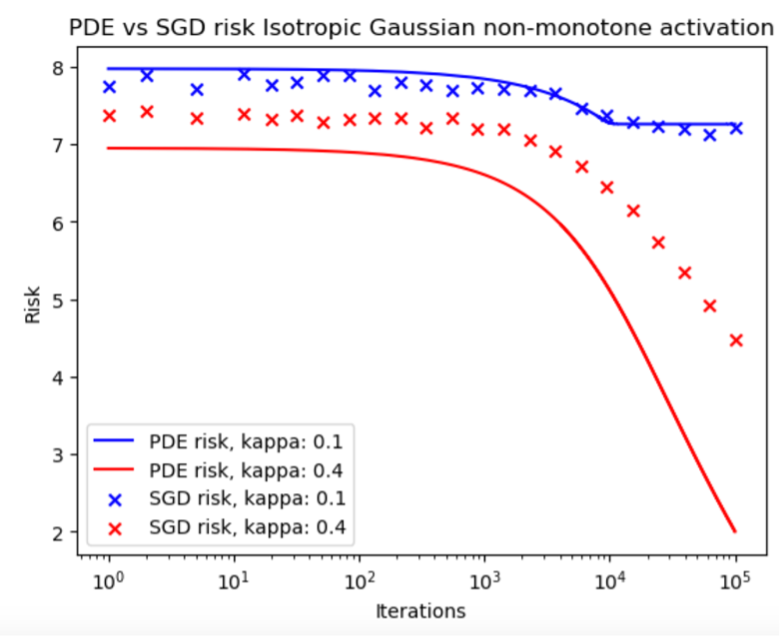
\includegraphics[width=0.8\linewidth]{images/NGuyen2018-pde-sgd-risk-iso-gauss-non-mon.png}
  \caption{Plot comparing PDE vs SGD risk for the\\  non-monotone activation $ \sigma$.}
  \label{fig: pde vs sgd non-monotone}
\end{subfigure}%
\begin{subfigure}{0.5\textwidth}
  \centering
  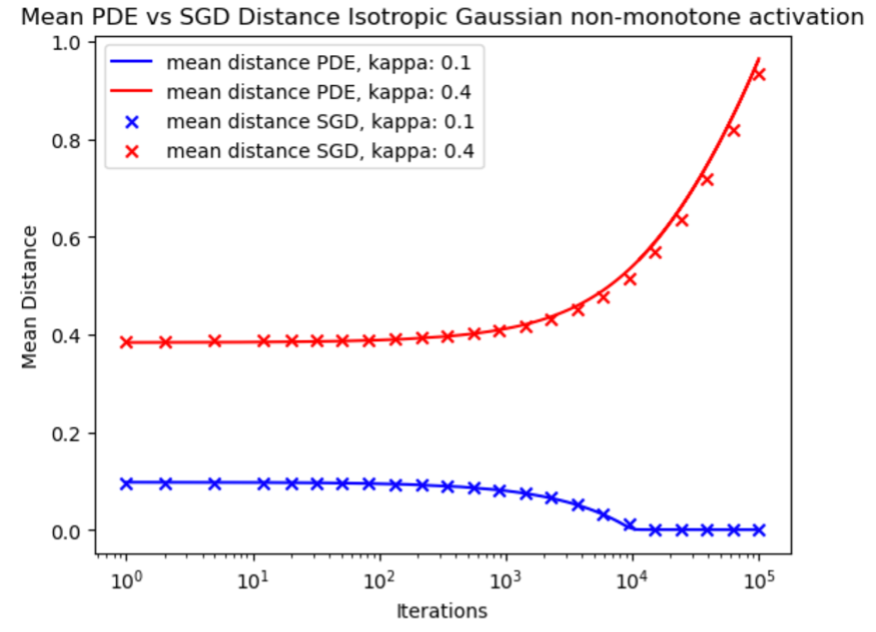
\includegraphics[width=0.8\linewidth]{images/NGuyen2018-pde-sgd-iso-gauss-non-mon.png}
  \caption{ Plot comparing the average distance of the weights $ \norm{w}_{2}$ in the PDE vs SGD simulations for the non-monotone activation.}
  \label{fig:  avg distance pde sgd non-monotone}
\end{subfigure}
\caption{ Separating two isotropic Gaussians, with a non-monotone activation function $ \sigma$. Here $N = 800, d = 320, \Delta = 0.5$. Continuous lines are prediction
obtained with the Distributional Dynamics simplified to reflect the spherical symmetry of the problemS.
}
\label{fig:  non-monotone simulation sgd vs pde}
\end{figure}


\subsection{Anisotropic Gaussians}

I also implemented code for SGD and PDE simulations of risk for the non-isotropic Gaussian case of failure of SGD given two initializations motivated by the theory developed in \cite{Mei_2018}. The PDE simulations reproduce the numerical findings in the paper, but SGD runs fail to match the PDE profiles exactly, though qualitatively, they are similar (figure \ref{fig: anisotropic gaussian case plots}. More precisely, the data is now 
\begin{equation}
\begin{array}{cc}
& \text{with probability}  1/2: y = +1, \mathbf{x}\sim N(0, \Sigma_+)\\
& \text{with probability}  1/2: y = -1, \mathbf{x}\sim N(0, \Sigma_-)
\end{array}
\end{equation}
where 
\begin{equation}
\begin{array}{cc}
	\Sigma_+ &= \text{Diag}(\underbrace{(1+\Delta)^{2}, \cdots, (1+\Delta)^{2}}_{s_0}, \underbrace{1,\cdots, 1}_{d-s_0})\\ 
 \Sigma_- &= \text{Diag}(\underbrace{(1-\Delta)^{2}, \cdots, (1-\Delta)^{2}}_{s_0}, \underbrace{1,\cdots, 1}_{d-s_0})
\end{array}
\end{equation}
and as in the previous case, we choose $\sigma_*(\mathbf{x};\mathbf{\theta}_{i})=a_{i}\sigma_{\text{ReLU}}(\bracket{\mathbf{x}}{w_{i}}+b_{i})$  where $ \sigma_{\text{ReLU}}(x) = \max{x,0}$.

     \begin{figure}[H]
 \begin{subfigure}{0.5\textwidth}
   \centering
   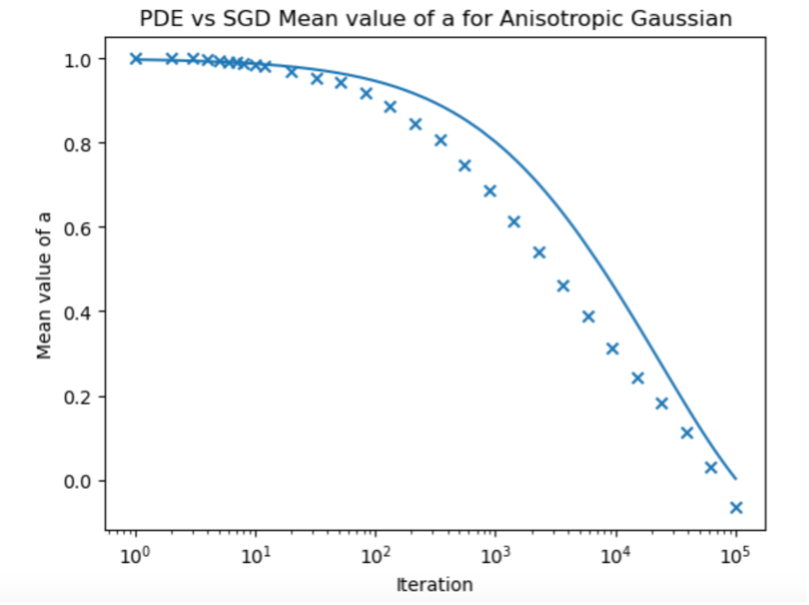
\includegraphics[width=0.8\linewidth]{images/NGuyen2018-pde-sgd-gauss-anisotropic.png}
   \caption{Mean value of $ a$ for PDE and SGD in the anisotropic Gaussian case.}
   \label{fig: val a anisotropic}
 \end{subfigure}%
 \begin{subfigure}{0.5\textwidth}
   \centering
   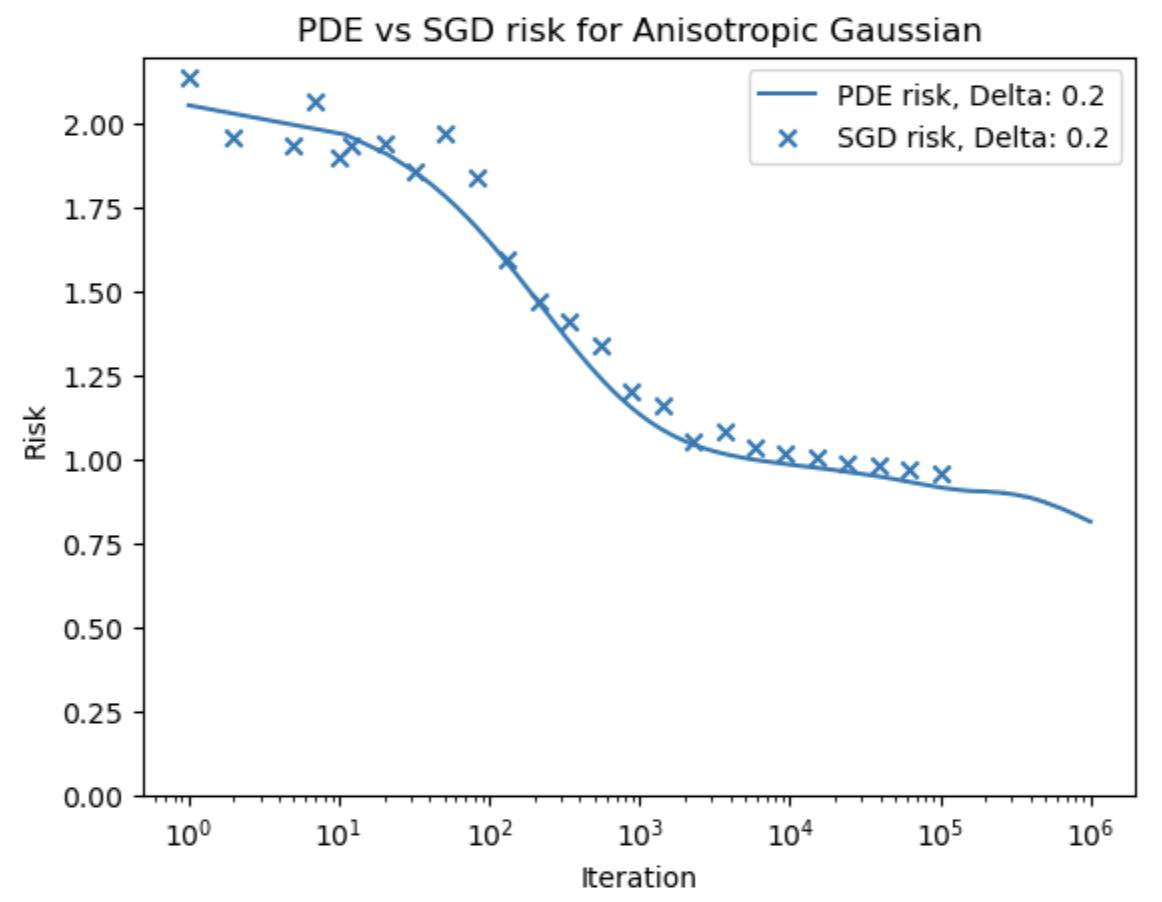
\includegraphics[width=0.8\linewidth]{images/NGuyen2018-pde-sgd-risk-gauss-anisotropic.png}
   \caption{PDE vs SGD risk for Anisotropic Gaussian}
   \label{fig: risk anisotropic}
 \end{subfigure}
 \caption{ caption}
 \label{fig: anisotropic gaussian case plots}
 \end{figure} 

\subsection{MNIST data classification}

I studied the proofs for the propagation of chaos and the mean-field limit of the distribution of neural network weights in the 2019 paper of Spiliopoulos and Sirgiano entitled ‘Mean Field Analysis of Neural Networks: A Law of Large Numbers’ and its companion paper \cite{sirignano2019meanfieldanalysislln}, \cite{sirignano2019meanfieldanalysisclt}. I did some background reading to supplement my understanding of the above papers of a book entitled ‘Markov Processes: Characterization and Convergence’ by Stewart N. Ethier, Thomas G. Kurtz \cite{ethier2009markov}, specifically the chapter on weak convergence of probability measures with values in Skorokhod spaces defined below.

\begin{boxdef}[Skorokhod space]\label{def: skorokhod}
	Let $  E = (\mathcal{M}, d)$ be a metric space and $ T>0$. Then, we deefine the \underline{Skorokhod space} 
\begin{equation}
	\mathcal{D}([0,T]; E) \coloneqq \{f:[0,T]\to E: f \text{ is cadlag}\}.
\end{equation}

\end{boxdef}

This mean field convergence of the empirical measures induced by the weights of neural networks was also performed in papers \cite{sirignano2019meanfieldanalysisclt} and \cite{sirignano2019meanfieldanalysislln}. In a similar setup to \cite{Mei_2018}, the SGD algorithm produces obtains empirical measures expended in a piewewise constant manner to $\mu^{N}_{t} = \hat{\rho}^{N}_{\lfloor Nt \rfloor}$ for $ t\geq 0$, see figure \ref{fig: piecewise constant extension of function}. 
\begin{figure}[H]
    \centering
    \includesvg[width=0.6\textwidth]{images/piecewise-constant.svg}
    \caption{Piecewise constant extension of scaled empirical measures $ \mu^{N}_{t}$.}
    \label{fig: piecewise constant extension of function}
\end{figure}

Now, by construction, we have that the empirical measure process $ (\mu^{N}_{t})_{t\in [0,T]}$ is an element of the space of locally finite Borel measures on $ \R^{d}$, $ \mathcal{M}(\R)^{d}$. One can define the notion of \textit{vague convergence} of a family $ (\nu_{n})_{n\in \N} \stackrel{v}{\to} \nu\in \mathcal{M}(\R^{d})$ by 

\begin{equation}\label{eq: vague conv}
	\int_{\R^{d}}f \diff \nu_{n}\stackrel{n\to \infty}{\to} \int_{\R^{d}}f \diff \nu_{n} \quad  f\in \hat{\mathcal{C}}(\R^{d}).
\end{equation}
where $ \hat{\mathcal{C}}_(\R^{d})$ denotes the space of all bounded continuous non-negative functions with bounded support. Note that the family of maps $\{\pi_{f}:f\in \hat {\mathcal{C}}_{\R^{d}}\} $ induces the vague topology $ \mathcal{T}$: 

\begin{boxlemma}[Vague topology on $  \mathcal{M}_{ \mathcal{S}}$]\label{lemma: vague topology}
Let $  \mathcal{S}$ be a complete separable metric space, then there exists a topology $  \mathcal{T}$ on $  \mathcal{M}_{ \mathcal{ S}}$ such that
\begin{enumerate}
\item $ \mathcal{T}$ induces the convergence $ \nu_{n}\stackrel{v}{\longrightarrow}\nu$ in \ref{eq: vague conv},
\item $ \mathcal{M}_{ \mathcal{S}}$ is Polish under $  \mathcal{T}$,
\item $  \mathcal{T}$ generates the Borel sigma algebra $\sigma(\{\pi_{f}:f\in \hat {\mathcal{C}}_{\R^{d}}\})$.
\end{enumerate}

\end{boxlemma}

Hence, we have that the scaled empirical measure $ (\mu^{N}_{t})_{t\in [0,T]})$ is a random element of $ \mathcal{D}_{ \mathcal{M}(\R)^{d}} \coloneqq \mathcal{D}([0,T]; ( \mathcal{M}(\R^{d}), d_\mathcal{T}))$, where $d_ \mathcal{T}$ is the induced metric from \ref{lemma: vague topology}. Note that $  \mathcal{D}_{ \mathcal{M}(\R)^{d}}$ space is a Polish space in its own space endowed with the \textit{Skorokhod topology} with well-understood criteria for compactness that feature prominently in the proof of the main theorem in \cite{sirignano2019meanfieldanalysislln}, and \cite{sirignano2019meanfieldanalysisclt}.\\

The main result of the paper \cite{sirignano2019meanfieldanalysislln} concerns the convergence in distribution of $ \mu^{N}_{t}$ in the aforementioned Skorokhod space under certain `reasonable` structural assumptions.

\begin{theorem}[Spiliopoulos LLN]\label{thm: spilopoulos lln}
	For all $ T>0$, the scaled empirical measure $ \mu^{N}_{t}$ on $ [0,T]$ converges in distribution to a
 limit measure $ \bar{\mu}_{t}$ with values in $  \mathcal{D}_{\mathcal{M}_{\R^{d}}} $ as $ N\to \infty$.
\end{theorem}

\begin{remark}
    $ \mu_{t}$ has a characterisation as the unique deterministic weak solution to a PDE, interpeted in the weak sense. Also, since the limiting measure $ \mu_{t}$ is deterministic for all $ t\geq 0$, we have the stronger convergence in Probability, that is for all $ \delta >0$
    \[
    \displaystyle \lim_{N\to \infty}\PP(d_{  \mathcal{D}_{\mathcal{M}_{\R^{d}}} }(\mu^{N}, \bar{\mu})\geq \delta) = 0 
    \]
    
\end{remark}


Moreover, I read the companion paper of Spiliopoulos (2019) \cite{sirignano2019meanfieldanalysisclt} where the authors proved a CLT for a one-layer neural network. To this end, the authors in \cite{sirignano2019meanfieldanalysisclt} the fluctuation process 
\begin{equation}
	\eta^{N}_t = \sqrt{N}(\mu^{N}_{t}-\bar{\mu}_{t})
\end{equation}
The main result in \cite{sirignano2019meanfieldanalysisclt} is that asymptotically, as $ N\to \infty$, the fluctuations converge in distribution, in a way made precise below, to some measure-valued process $ \bar{\eta}$, where satisfies a stochastic partial differential equation. This result achieves to give a characterisation of the fluctuations of the finite empirical measure $ \mu^{N}$ around its mean-field limit $ \bar{\mu}$ for large $ N$ . It is noted that the $ \bar{\eta}$
has a Gaussian distribution.

\begin{theorem}[Spiliopoulos CLT]\label{thm: spiliopoulos CLT}
	Under the 'reasonable' assumptions outlined in \cite{sirignano2019meanfieldanalysisclt}, $J \geq 3\left \lceil \frac{d}{2}\right\rceil+7$ and any $ 0<T<\infty$. The sequence
	\begin{equation} 
		((\eta^{N}_{t})_{t\in [0,T]})_{N\in \N}\stackrel{d}{\to} ((\bar{\eta}_{t})_{t\in [0,T]})_{N\in \N}
	\end{equation}
	in $\mathcal{D}([0,T];W^{-J,2}), \text{ as } \N\to \infty$ where $ W^{-J,2}$ is the space of all continuous linear functionals on the \textit{Sobolev space} $ W^{J,2}_{0}(\Theta)$, where $ \Theta\subseteq\R^{d}$ is a bounded domain independent of $ N$.
\end{theorem}

\begin{remark}
	For a brief introduction into the Sobolev spaces mentioned above, refer to section $ 2$ to in \cite{sirignano2019meanfieldanalysisclt}.
\end{remark}


Furthermore, regarding the paper of Spiliopoulos (2019) on the LLN for the one-layer neural net \cite{sirignano2019meanfieldanalysislln}, I implemented a single-digit classifier with the architecture satisfying the assumptions made in the paper and was able to reproduce the distribution of parameters in the paper.

\begin{figure}[H]
    \centering
    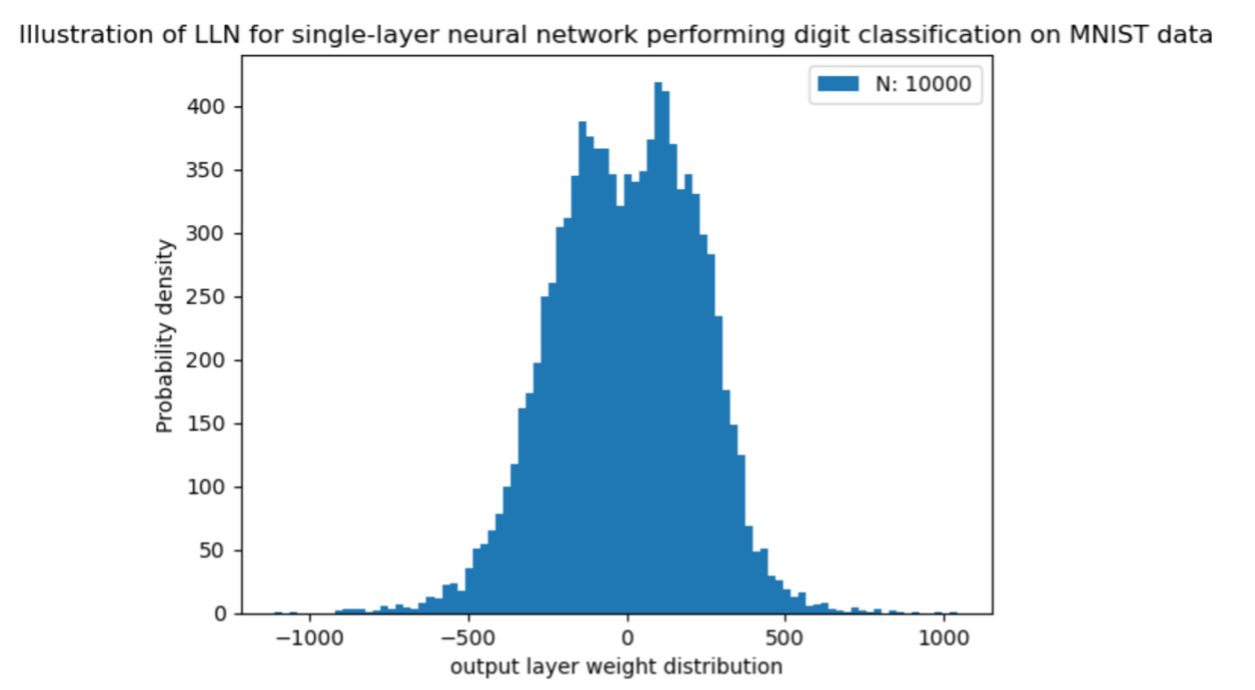
\includegraphics[width=0.8\textwidth]{images/Spiliopoulos2019-LLN-singleNN-mnist.png}
    \caption{weights of MNIST single digit classification single layer neural net}
    \label{fig: MNIST spiliopoulos}
\end{figure}

\section{Non-convex landscape}

\subsection{Approaches}

At this point in the project, the focus started to shift from the theoretical mean-field analysis of neural network algorithms towards studying possible approaches to alleviate the failure of SGD to reach a global minimum by potentially getting stuck in very sharp, yet non-global minima when the potential is wildly non-convex.\\ 

In this direction, I read my supervisor's paper on shallow minima: ‘The sharp, the flat and the shallow: Can weakly interacting agents learn to escape bad minima?’, \cite{kantas2019sharpflatshallowweakl}. In thie paper, the authors review several variants of SGD and illustrate that a system of interacting, rather than i.i.d., agents (essentially an interacting particle system) performing gradient descent can help to smooth out sharp minima and thus implicitly convexify
the loss function.\\ 

The setting is a modification of the Stochastic Gradient Langevin Dynamics (SGLD) framework:
\begin{equation}\label{eq: SGLD}
	\diff X_{t} = -\nabla \Phi(X_{t})\diff t + \sqrt{2}\betadfB_{t}, \quad X_{0}\sim \eta_{0}
\end{equation}
where $ \Phi$ the loss function $ B_{t}$ is a standard Brownian motion and $ \eta_{0}$ is the initial distribution.

Three approaches are discussed before a synthesis of the last two yields their proposed algorithm, see \ref{alg: mf hom sgld}.



\subsubsection{Regularise potential directly by convolution}\label{sec:direct smoothing}

To eliminate sharp local minima one could replace the gradient term
in the basic gradient descent algorithm with a smoother version. In order to
eliminate these local minima one could simulate the gradient descent
dynamics of a ``smoothed'' version of the cost function instead
\begin{equation}
dX_{t}=-\nabla\Phi^{h}(X_{t})dt\label{eq:ode_h}
\end{equation}
where we denote 
\begin{equation}
\Phi^{h}\left(y\right)=(G_{h}\star\Phi)(y)=\int G_{h}(y-x)\Phi(x)dx,\label{eq:integrate phi}
\end{equation}
i.e. $\star$ denotes the convolution. A typical choice for the smoothing
kernel $G_{h}$ is the Gaussian kernel with variance $h$ 
\[
G_{h}(z)=\frac{1}{\left(2\pi h\right)^{d/2}}\exp\left(-\frac{\left\Vert z\right\Vert ^{2}}{2h}\right).
\]
For technical conditions for the above modification of the gradient, see the references in \cite{kantas2019sharpflatshallowweakly}. Regardless
of the choice of the smoothing kernel, $\Phi^{h}$ can be interpreted
as an expectation 

\[
\Phi^{h}\left(x\right)=\int\Phi(x+y)\mu(dy),
\]
for a suitably chosen probability measure $\mu$. Furthermore, (under
appropriate conditions) 
\begin{equation}
\nabla\Phi^{h}\left(x\right)=\int\nabla\Phi(x+y)\mu(dy).\label{eq:smooth_grad}
\end{equation}
An additional point here is that when $y\sim\mu$, $\nabla\Phi(x+y)$
is an unbiased estimate of the ``biased'' gradient $\nabla\Phi^{h}$.
This implies, in particular, that there is an additional option for
randomization of the smoothed gradient.\\ 

Loosely speaking the effect of $\mu$ here is to smooth $\Phi$.
It is natural to ask how one designs $\mu$ (or $G_{h}$)
to get the desired effect of smoothing of $\Phi$. There a multiple complications with such an approach, a pressing one being that computing the integral in \ref{eq:integrate phi}
for the type of loss functions that appear in machine learning applications
is intractable. To help mitigate these issues, the authros look at approaches where a smoothing measure $\mu$ does not act directly on $\Phi$ and is constructed from the stochastic process itself.
%%%%%%%%%%%%%%%%%%%%%%%%%%%%%%%%%%%%%%%%%%%%%%%%%%%%%%%%%


\subsubsection{Regularise the potential implicitly weakly interacting agents}\label{sec: weakly interacting agents}

Next, I studied variants of \ref{eq: SGLD} so that the
process $X_{t}$ will eventually end up closer to a minimizer of $\Phi$ with the rate of convergence taken into account. It is known that the law of the diffusion process $X_{t}$
has a smooth density with respect to the Lebesgue measure that satisfies
the Fokker-Planck (forward Kolmogorov) equation: 
\[
\partial_{t}\rho=\nabla\cdot\left(\rho\nabla\left(\beta\log\rho+\Phi\right)\right),\quad\rho(0,\cdot)=\eta_{0}(\cdot).
\]
Under appropriate relatively mild assumptions on the growth of the loss function $\Phi$
at infinity, the density $\rho$ converges exponentially fast in relative
entropy (Kullback-Leibler divergence) to the unique stationary state
\[
\rho_{\infty}=\frac{1}{Z}\exp(-\beta\Phi(x)),
\]
(see for instance \cite[Ch. 4]{pavliotis2014stochastic}) where $Z$ denotes the normalization constant.
Finding the mode or maximiser of $\rho_{\infty}$ is equivalent finding
$x^{*}$ (the minimizer of $ \Phi$). Here it is noted that higher values of $ \beta$
result to $\rho_{\infty}$ putting more of its mass around lower valued
local minima of $\Phi$. For high $\beta$, the SGLD \ref{ eq: SGLD}
reduces to a deterministic gradient descent, so it could be harder
to escape from local minima. In practice, the trade-off between convergence
speed and optimality is difficult to balance.

An alternative approach is to use interacting SGLD, as opposed to
i.i.d. copies of the Langevin dynamics~\ref{ eq: SGLD}. In \cite{kantas2019sharpflatshallowweakly}, a system of interacting SGLD of the form 
\begin{align}
dX_{t}^{i} & =-\nabla\Phi(X_{t}^{i})dt-\big(\nabla D\star\eta_{t}^{N}\big)(X_{t}^{i})dt+\sqrt{2\beta^{-1}}dB_{t}^{i},\label{eq:interacting_sde}
\end{align}
where $i=1,\ldots,N,$ $\eta_{t}^{N}=\frac{1}{N}\sum_{i=1}^{N}\delta_{X_{t}^{i}}$,
$X_{0}^{i}\sim\eta_{0}(\cdot)$. Compared to the i.i.d. SGLD \ref{ eq: SGLD},
the dynamics \ref{eq:interacting_sde} uses $D(x,y)$ as an interaction
potential, which, in this paper, we will take to be convex. In particular,
we will consider the so-called Curie-Weiss interaction
\begin{equation}
D(x,y)=\frac{\lambda}{2}\|x-y\|^{2}\label{e:inter}
\end{equation}
so that each particle experiences a linear attractive (mean reverting)
force to the empirical mean of all particles 
\[
\nabla D\star\eta_{t}^{N}(X_{t}^{i})=\lambda\left(X_{t}^{i}-\frac{1}{N}\sum_{j=1}^{N}X_{t}^{j}\right).
\]

The framework developed here can be conceived of as an abstraction of popular
machine learning algorithms, with ample references made in the paper \cite[p. 4]{kantas2019sharpflatshallowweaklSy}.\\

Under appropriate assumptions
on the loss function, and on the initial conditions the position of
each agent converges, in the limit $N\rightarrow\infty$ to the solution
of the McKean SDE 
\begin{align*}
d\bar{X}_{t} & =-\nabla\Phi(\bar{X}_{t})dt-\nabla D\star\eta_{t}(\bar{X}_{t})dt+\sqrt{2\beta^{-1}}dB_{t},\\
\eta_{t} & =\mathcal{L}aw\left(\bar{X}_{t}\right).
\end{align*}
The density of the law of the process $\bar{X}_{t}$ is given by the
McKean-Vlasov equation: 
\begin{equation}
\partial_{t}\eta=\nabla\cdot\left(\eta\nabla\left(\beta\log\eta+\Phi+D\star\eta\right)\right),\quad\eta(0,\cdot)=\eta_{0}(\cdot).\label{e:mc-vl}
\end{equation}

This approach uses $\Phi+D\star\tilde{\eta}$ instead of $\Phi$ and acts to regularise
or smooth out the cost function. From an optimization point of view,
substituting $-\nabla\Phi(x)-\nabla D\star\eta_{t}^{N}(x)$ and using
a linear interaction for $\nabla D$ is equivalent to using an $\ell_{2}$-penalty
in the objective function for the constraint: $X_{t}^{i}=\frac{1}{N}\sum_{j=1}^{N}X_{t}^{j}$,
for each agent $i$. Therefore, for an appropriate choice of the interaction
strength $\lambda$, the objective function is approximately convex.

\subsubsection{Homogenisation}

In the previous section \ref{sec: weakly interacting agents} the empirical measure $\eta_{t}^{N}$ was used
to smooth the potential based on empirical properties of interacting
agents. In this section, the approach that
was developed in \cite{Chaudhari2017DeepRP} to convert \ref{eq: SGLD}
into the following gradient descent algorithm: 
\begin{equation}
d\tilde{X}_{t}=-\nabla\Phi^{\beta,\gamma}(\tilde{X}_{t})dt,\quad\Phi^{\beta,\gamma}\left(x\right)=\int\Phi(x-y)\rho_{\infty}^{x}(dy),\label{eq:hom_sde_lim}
\end{equation}
is briefly discussed, where $\rho_{\infty}^{x}$ is the invariant measure of $Y_{t}$ that
appears in the limit when $\epsilon\rightarrow0$ for the following
fast/slow SDE system \begin{subequations}\label{eq:hom_sde_v2} 
\begin{align}
dX_{t} & =-\nabla\Phi(X_{t}-Y_{t})dt\label{eq:hom_sde_v2_1}\\
dY_{t} & =-\frac{1}{\epsilon}\left(\frac{1}{\gamma}Y_{t}-\nabla\Phi(X_{t}-Y_{t})\right)dt+\sqrt{\frac{2\beta^{-1}}{\epsilon}}dB_{t}\label{eq:hom_sde_v2_2}
\end{align}
\end{subequations}The parameter $\epsilon$ measures scale separation.
The limit $\epsilon\rightarrow0$ can be justified using multiscale
analysis. Note that this is a gradient
scheme for the modified loss function $\Phi(x-\frac{y}{\epsilon})+\frac{1}{2\gamma}\left\Vert \frac{y}{\epsilon}\right\Vert ^{2}$.
It is noted in \cite{kantas2019sharpflatshallowweakly} that $\gamma$ acts as a regularization parameter,precisely like the inverse of the interaction strength $\lambda$
in the previous section. We emphasize the similarities between~\ref{eq:integrate phi}
and \ref{eq:hom_sde_lim}.

It is important to note that the smoothed loss function in \ref{eq:hom_sde_lim}
can also be calculated via convolution with a Gaussian kernel: 
\begin{equation}
\Phi^{\beta,\gamma}(x)=\frac{1}{\beta}\log\Big(G_{\beta^{-1}\gamma}\star\exp(-\beta\Phi)\Big).\label{e:phi-cole-hopf}
\end{equation}
This is the Cole-Hopf formula for the solution of the viscous Hamilton-Jacobi
equation with the loss function $\Phi$ as the initial condition,
posed on the time interval $[0,\gamma]$. The larger $\gamma$ is,
the more regularized the effective potential (or relative entropy)
$\Phi^{\beta,\gamma}(x)$ is. \\ 

Importantly for the authors in \cite{kantas2019sharpflatshallowweakly}, in~\cite{Chaudhari2017DeepRP} an equivalent formulation
to~\ref{eq:hom_sde_v2}: \begin{subequations}\label{eq:hom_sde}
\begin{align}
dX_{t} & =-\frac{1}{\gamma}(X_{t}-Y_{t})dt\label{eq:hom_sde1}\\
dY_{t} & =-\frac{1}{\epsilon}\left(\nabla\Phi(Y_{t})-\frac{1}{\gamma}(X_{t}-Y_{t})\right)dt+\sqrt{\frac{2\beta^{-1}}{\epsilon}}dB_{t}.\label{eq:hom_sde2}
\end{align}
\end{subequations} Here the regularized cost appears as $\Phi(\frac{y}{\epsilon})+\frac{1}{2\gamma}\left\Vert x-\frac{y}{\epsilon}\right\Vert ^{2}$.
This form is more convenient for the numerical implementation and
is the one that will be used in Algorithm \ref{alg: mf hom sgld}.


\subsubsection{Synthesis: combine both multi-scale analysis and weakly interacting gents for MF Hom SGLD}
In brief this algorithm, \ref{alg: mf hom sgld} corresponds to a discretization of the dynamics of gradient descent against a potential with an $ \ell_{2}$ penalty and a regularized version of the original potential $\Phi$, using the method introduced by Chaudhari et al. (2018).

More precisely, combining~\ref{eq:hom_sde_lim} with \ref{eq:interacting_sde}
we obtain: 
\begin{align}
dX_{t}^{i} & =-\frac{1}{\gamma}(X_{t}^{i}-Y_{t}^{i})dt-\lambda\left(X_{t}^{i}-\frac{1}{N}\sum_{j=1}^{N}X_{t}^{j}\right)dt\label{eq:hom_mf_sde1}\\
dY_{t}^{i} & =-\frac{1}{\epsilon}\left(\nabla\Phi(Y_{t}^{i})-\frac{1}{\gamma}(X_{t}^{i}-Y_{t}^{i})\right)dt+\sqrt{\frac{2\beta^{-1}}{\epsilon}}dW_{t}^{i}\label{eq:hom_mf_sde2}
\end{align}
This scheme was tested numerically in the context of learning for the single layer neural network (see Section \ref{sec: neural net single layer}) with a sufficiently small value of $\epsilon$,
to approximate better the homogenized limit, as per \cite{kantas2019sharpflatshallowweakly}. The theoretical justification of this algorithm requires the study of the joint limits $\epsilon\rightarrow0$
and $N\rightarrow+\infty$ (see \cite[p. 6]{kantas2019sharpflatshallowweakly} for details and references). \\ 


To discretize \ref{eq:hom_mf_sde1}-\ref{eq:hom_mf_sde2} effectively
for small $\epsilon$ I followed \cite{kantas2019sharpflatshallowweakly} and used the heterogeneous multiscale method \cite{weinan2005analysis} in Algorithm \ref{alg: mf hom sgld}:

\begin{examplesblock}{MF Hom SGLD}\label{alg: mf hom sgld}
\begin{algorithmic}
	\Require $\mathsf{X}_{0}^{i}\sim\eta_{0}, \lambda \sim 1 \Delta >0$ \Comment{ $ \Delta$ is a step size}
\For{$n\geq 1, i=1,\ldots,N$}
\State Set $\mathsf{Y}_{n,0}^{i}=\mathsf{Y}_{n-1,m'+M-1}^{i}$;
\For{$m=1,\ldots,M$}  
\State \[\begin{array}{ll}
	\mathsf{Y}_{n,m}^{i} &=\mathsf{Y}_{n,m-1}^{i}-\frac{\delta}{\epsilon}\left(\nabla\Phi(\mathsf{Y}_{n,m-1}^{i})-\frac{1}{\gamma}(\mathsf{X}_{n-1}^{i}-\mathsf{Y}_{n,m-1}^{i})\right)\\&+\sqrt{\frac{2\beta^{-1}\delta}{\epsilon}}Z_{n,m}^{i};\:Z_{n,m}^{i}\sim N(0,I).
\end{array}\]
\EndFor
\State Compute average $\mathcal{Y}_{n}^{i}=\frac{1}{(m'+M-1)}\sum_{m=m'}^{m'+M-1}\mathsf{Y}_{n,m-1}^{i}$
\State Update
 \State  
\begin{align*}
\mathsf{X}_{n}^{i} & =\mathsf{X}_{n-1}^{i}-\frac{1}{\gamma}(\mathsf{X}_{n-1}^{i}-\mathcal{Y}_{n}^{i})\Delta-\lambda\left(\mathsf{X}_{n-1}^{i}-\frac{1}{N}\sum_{j=1}^{N}\mathsf{X}_{n-1}^{i}\right)\Delta
\end{align*}
\EndFor 
\end{algorithmic}
\end{examplesblock}

\subsubsection{Nesterov SGD}

\begin{examplesblock}{Nesterov SGD}\label{alg: nesterov sgd}
\begin{algorithmic}
    \State make connection to regularisation
\end{algorithmic}

\end{examplesblock}

\subsection{Applications}

\subsubsection{Muller Brown Potential}

Having developed some theory regarding modifications to the vanilla SGD for non-convex landscapes, we applied it to the canonical example, at least from chemistry \cite{muller1979location} of the Muller-Brown potential 
\begin{equation}
	V(x,y) = \displaystyle\sum^{4}_{i=i}A_{i}\cdot \exp[a_{i}\cdot(x-x_{0})^{2}+b_{i}\cdot(x-x_{0})+c_{i}\cdot(y-y_{0})+d_{i}\cdot (y-y_{0})^{2}] 
\end{equation}
where $A_{i}, a_{i}, b_{i}, c_{i}, d_{i}, i\leq 4$ are as in the paper \cite{muller1979location}. This potential has multiple local minima in close proximity, making it difficult for SGD to converge to the global minimum, see \ref{fig: muller-brown 3d}.

    \begin{figure}[H]
\begin{subfigure}{0.5\textwidth}
  \centering
  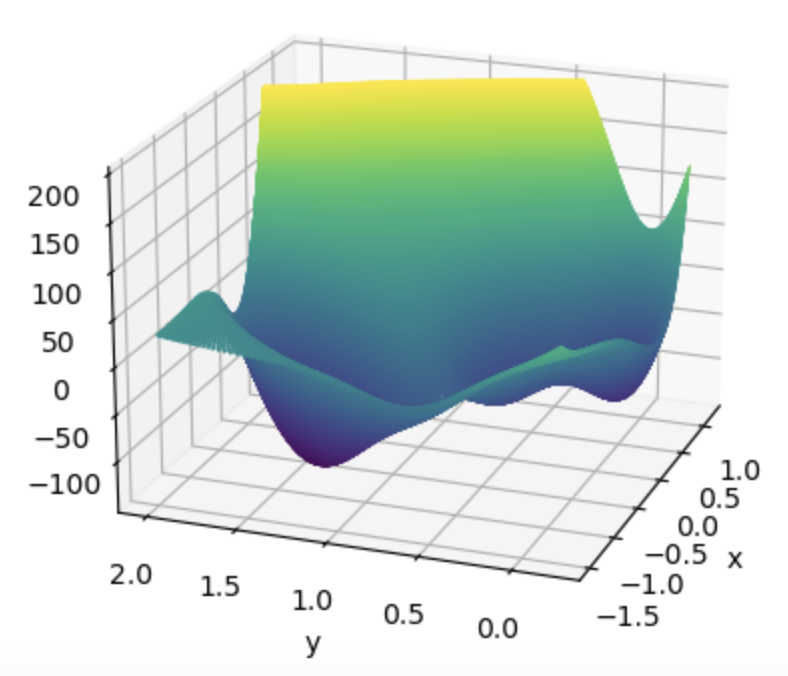
\includegraphics[width=0.8\linewidth]{images/MullerB-potential-plot-3d.png}
  \caption{3d plot of the Muller-Brown potential}
  \label{fig: muller-brown 3d}
\end{subfigure}%
\begin{subfigure}{0.5\textwidth}
  \centering
  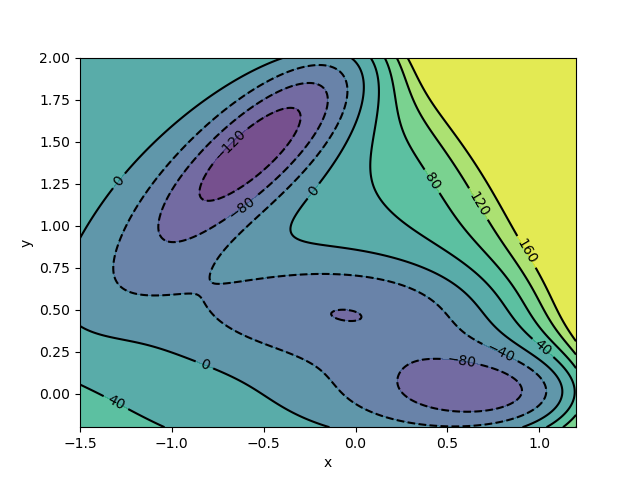
\includegraphics[width=0.8\linewidth]{images/MullerB-contour-with-grad-field.png}
  \caption{ caption}
  \label{fig:  muller-brown contour}
\end{subfigure}
\caption{Contour plot of the Muller-Brown potential}
\label{fig:  muller-brown plots}
\end{figure}


•	Muller-Brown potential analysis:
o	- Most algorithms on the MB potential get stuck equally on two local minima, i.e. the global one (which is narrow) and the one with the next smallest local minimum
o	- Convolving with a solution to the heat equation does not improve performance as the narrow steep global minimum (as seen from the plot) is smeared out first thus giving no hope of real convergence, unless the algorithms is lucky with the initialisation
o	- The Hom-MF-SGLD works surprisingly well against all others since it performs a gradient flow of a regularised potential, where regularisation is done at the level of the gibbs measure
o	- Idea, sample points (to initialise GD) more judiciously, i.e. with gibbs measure (inspired by Andrew Stuart's paper ) by performing a gradient flow and use that 'educated guess as the initialisation of a gd algorithm. (e.g. Wasserstein gradient flow, i.e. sgd on log of Gibbs measure of potential, or affine invariant Wasserstein)
o	- This idea seems to perform better that all algorithms except the MF-Hom-SGLD algorithm
o	- Regularising using the HJB equation (essentially performed in the MF-Hom SGLD algorithm) is better suited to minima that are narrower compared to regularisation with the heat equation that destroys such peaks first (due to large curvature)
o	- Tried regularising wrt soln of HJB equation directly and apply nesterov's accelerated gd algorithm with gradient restarting

\begin{figure}\centering
\subfloat[legend]{\label{a}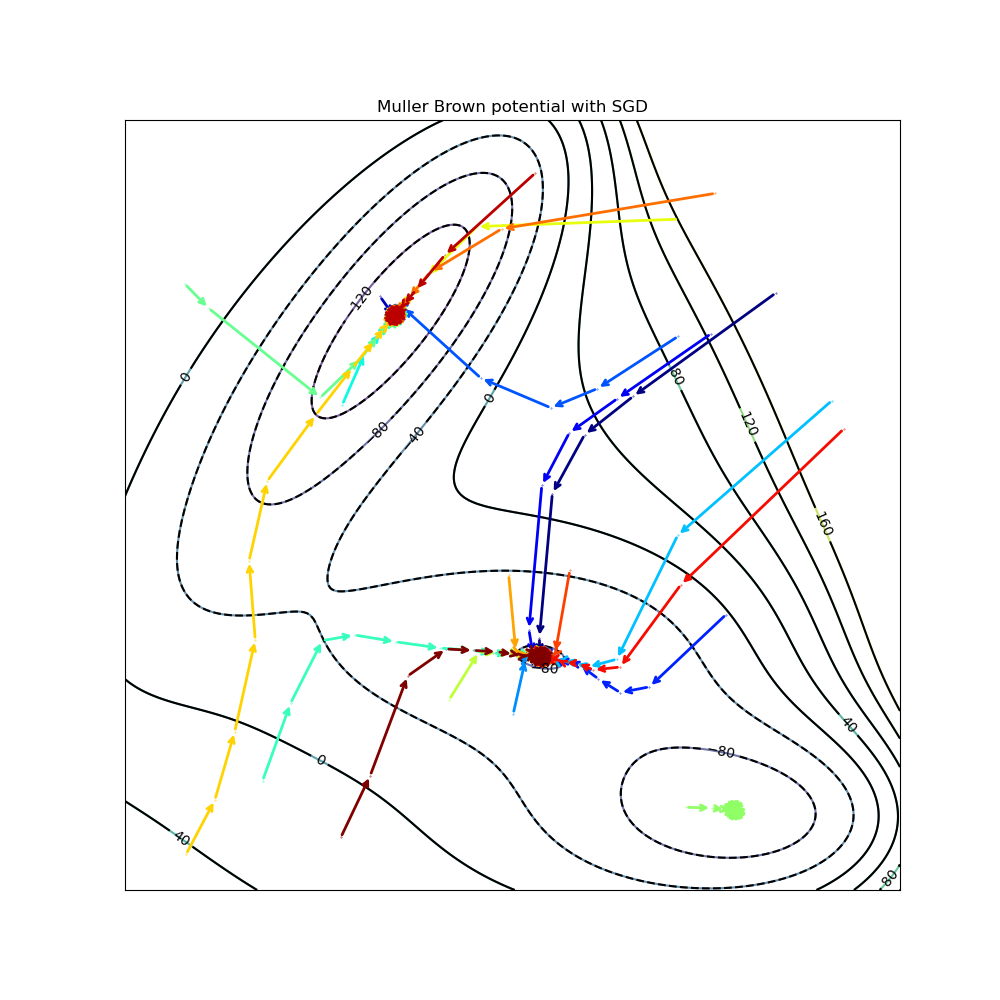
\includegraphics[width=.45\linewidth]{images/MullerBrown-SGD.png}}\hfill
\subfloat[legend]{\label{b}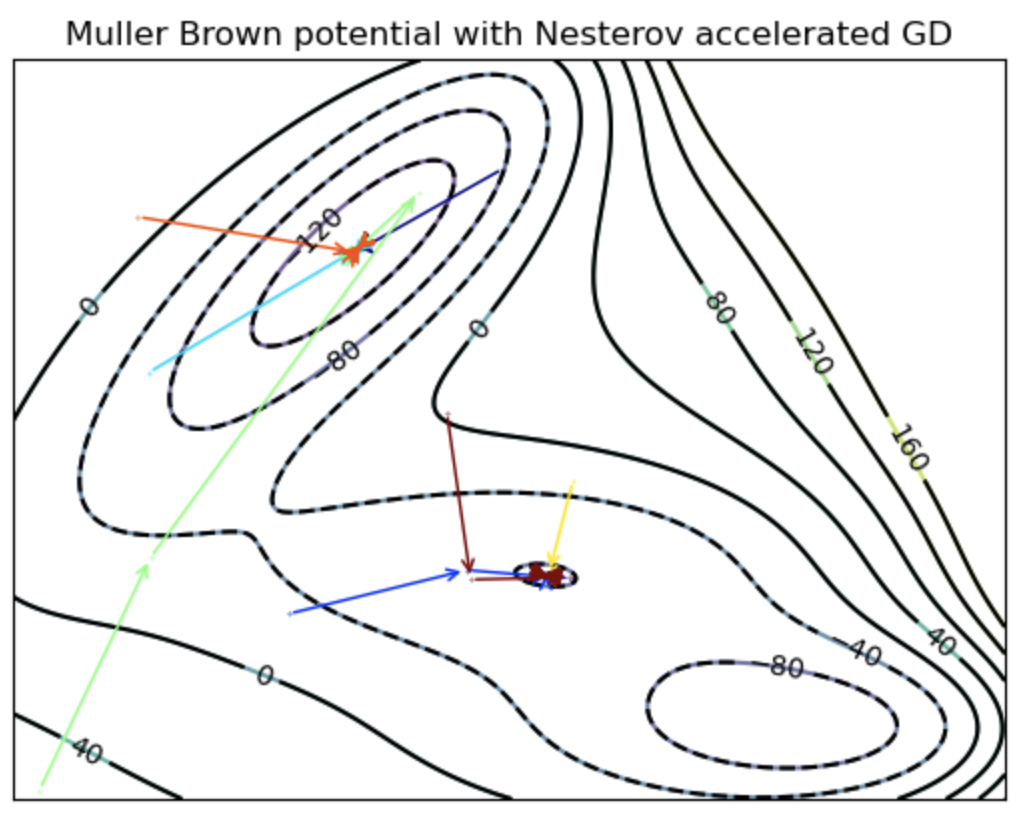
\includegraphics[width=.45\linewidth]{images/MullerB-NesterovSGD.png}}\par 
\subfloat[legend]{\label{c}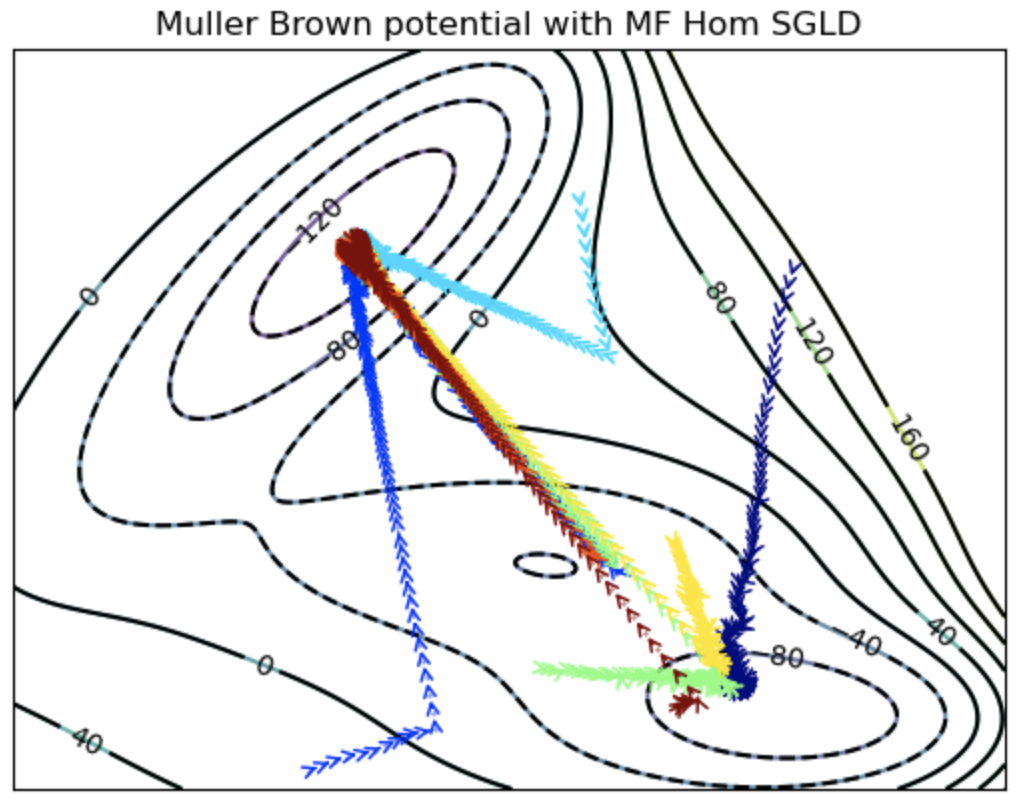
\includegraphics[width=.45\linewidth]{images/MullerBrown-HomSGLD.png}}
\caption{my fig}
\label{fig}
\end{figure}



\subsubsection{$ 3-$d spin model analysis}
"Neural networks, a central tool in machine learning, have demonstrated remarkable,
high fidelity performance on image recognition and classification tasks. These successes evince
an ability to accurately represent high dimensional functions, but rigorous results about the ap-
proximation error of neural networks after training are few. Here we establish conditions for global
convergence of the standard optimization algorithm used in machine learning applications, sto-
chastic gradient descent (SGD), and quantify the scaling of its error with the size of the network.
This is done by reinterpreting SGD as the evolution of a particle system with interactions governed
by a potential related to the objective or “loss” function used to train the network. We show that,
when the number n of units is large, the empirical distribution of the particles descends on a con-
vex landscape towards the global minimum at a rate independent of n, with a resulting approxima-
tion error that universally scales as O(n−1). These properties are established in the form of a Law
of Large Numbers and a Central Limit Theorem for the empirical distribution. Our analysis also
quantifies the scale and nature of the noise introduced by SGD and provides guidelines for the step
size and batch size to use when training a neural network. We illustrate our findings on examples in
which we train neural networks to learn the energy function of the continuous 3-spin model on the
sphere. The approximation error scales as our analysis predicts in as high a dimension as d = 25.\\

Read the van Eijnden paper and studied the proofs of asymptotic convergence to a gradient flow in the mean field limit and how this is preferable due to the convexification of the loss (as a functional of measures), similar to that observed in \cite{Mei_2018}.


To test our results, we use a function known for its complex
features in high-dimensions: the spherical 3-spin model,
$f: S^{d-1}(\sqrt{d}) \to \mathbb{R}$, given by
\begin{equation}
  \label{eq:psin}
  f(\mathbf{x}) = \frac1d \sum_{p,q,r=1}^d a_{p,q,r} x_p x_q x_r,  \qquad \mathbf{x}
  \in S^{d-1}(\sqrt{d}) \subset \mathbb{R}^d
\end{equation}
where the coefficients $\{a_{p,q,r}\}_{p,q,r=1}^d$ are independent
Gaussian random variables with mean zero and variance one. The
function~\eqref{eq:psin} is known to have a number of critical points
that grows exponentially with the dimensionality
$d$~\cite{Auffinger:2013kq,Sagun:2014tg,Auffinger:2012gh}. We note
that previous works have sought to draw a parallel between the glassy
3-spin function and generic loss
functions~\cite{Choromanska:2014ui}, but we are not exploring such an
analogy here. Rather, we simply use the function~\eqref{eq:psin} as a
difficult target for approximation by neural networks. That is,
throughout this section, we train networks to learn $f$ with a
particular realization of $a_{p,q,r}$ and study the accuracy of that
representation as a function of the number of particles $n$.

 \begin{figure}[H]\centering
\subfloat[legend]{\label{a}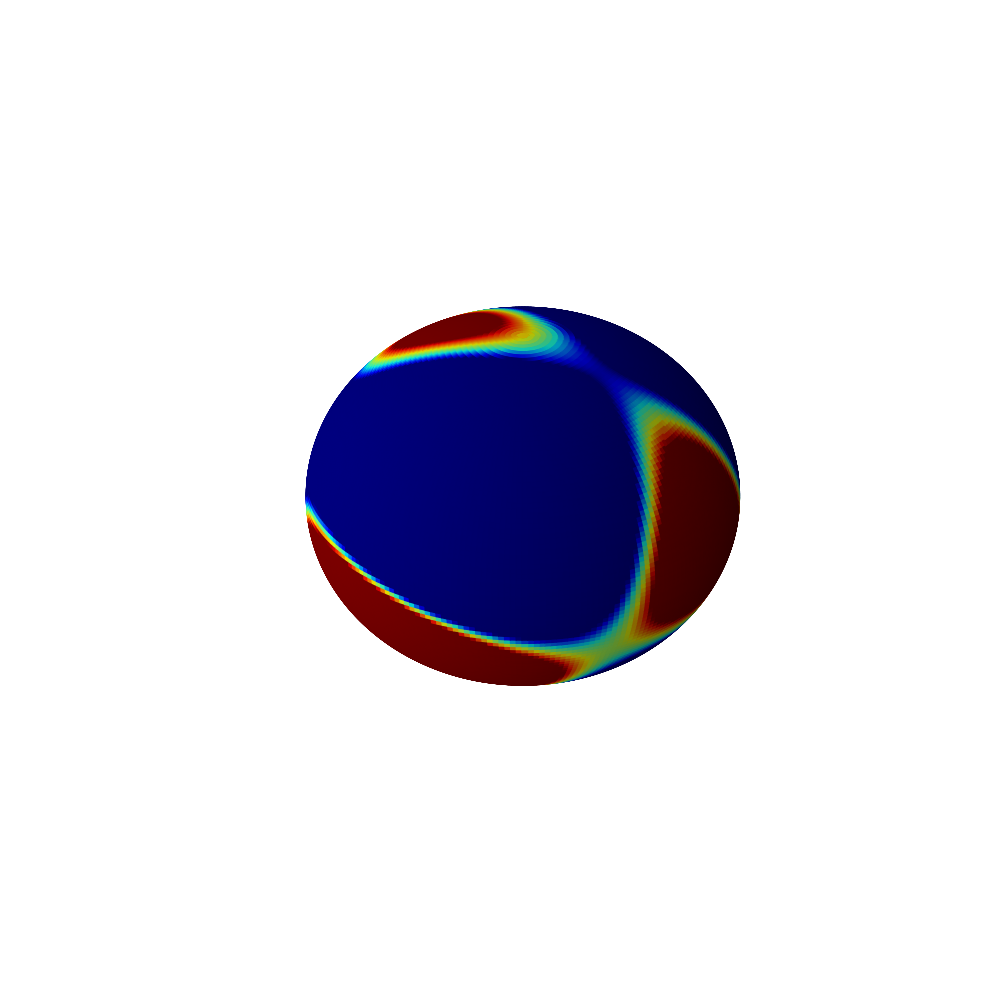
\includegraphics[width=.33\linewidth]{images/3d_spin_sphere_plot_d_3.png}}
\subfloat[legend]{\label{b}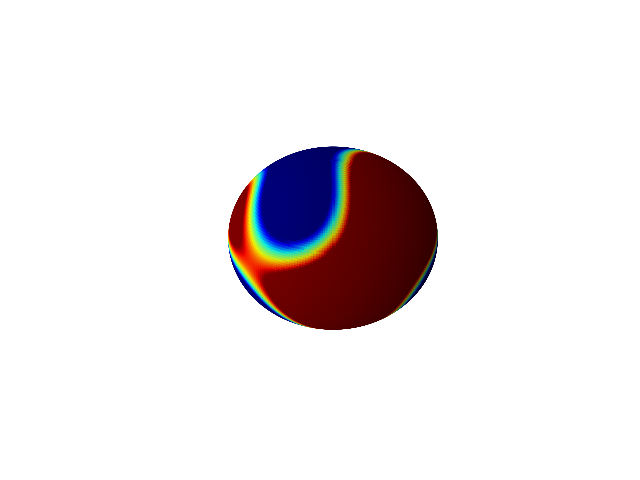
\includegraphics[width=.33\linewidth]{images/3d_spin_sphere_plot_d_4.png}}
\subfloat[legend]{\label{c}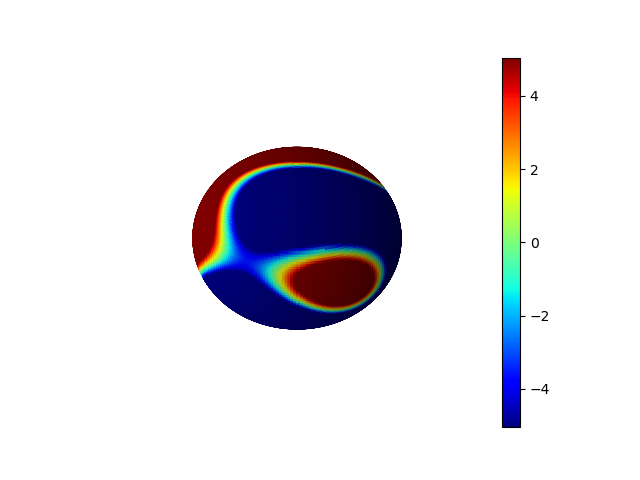
\includegraphics[width=.33\linewidth]{images/3d_spin_sphere_plot_d_5.png}}
\caption{my fig}
\label{fig}
\end{figure}

We first consider the case when $D = S^{d-1}(\sqrt{d})$ and we use
%
\begin{equation}
  \label{eq:90}
  \varphi(\mathbf{x},\mathbf{z}) = e^{-\tfrac12 \alpha |\mathbf{x}-\mathbf{z}|^2}
\end{equation}
%
for some fixed $\alpha >0$. In this case, the parameters
are elements of the domain of the function (here the $d$-dimensional
sphere). 
Note that, since $|\mathbf{x}|=|\mathbf{z}| = \sqrt{d}$, up to an
irrelevant constant that can be absorbed in the weights $c$, we can
also write~\eqref{eq:90} as
%
\begin{equation}
  \label{eq:90red}
  \varphi(\mathbf{x},\mathbf{z}) = e^{-\alpha \mathbf{x}\cdot \mathbf{z}}
\end{equation}
%
This setting allow us to simplify the problem. Using
%
\begin{equation}
  \label{eq:119}
  f^{(n)}(\mathbf{x}) = \frac1n \sum_{i=1}^n c_i \varphi(\mathbf{x},\mathbf{z}_i)
  = \frac1n \sum_{i=1}^n c_i e^{-\alpha \mathbf{x}\cdot \mathbf{z}_i},
\end{equation}

 To test the accuracy of the
representation, we used the following Monte Carlo estimate of the loss
function
%
 \begin{equation}
   \label{eq:lossempirical}
   \mathcal{L}_P[f^{(n)}_t] = \frac{1}{2P} \sum_{p=1}^P \left|f(\mathbf{x}_p) - f^{(n)}_t(\mathbf{x}_p)\right|^2.
 \end{equation}

 which is in close analogy to the risk \ref{eq: risk}
 This empirical loss function was computed with a batch of $10^6$
 points $\mathbf{x}_p$ uniformly distributed on the sphere.

We tested the representation~\eqref{eq:119} in $d=5$ using $n=16$, 32,
64, 128, and 256 and setting $\alpha = 5/d= 1$. The training was done
by running a time-discretized version of~\eqref{eq:34RBFpspin} with
time step $\Delta t = 10^{3}$ for $2 \times 10^5$ steps: during the
first $10^5$ we added thermal noise to
\eqref{eq:34RBFpspin}, which we then remove during the second half of
the run. The representation~\eqref{eq:119} proves to be accurate even
at rather low value of $n$: for example, the right panel of
Fig.~\ref{fig:5DRBF} shows a contour plot of the original function $f$
and its representation $f^{(n)}$ with $n=128$ through a slice of the
sphere defined as
%
\begin{equation}
  \label{eq:slice}
  \mathbf{x}(\theta) = \sqrt{d} \left(\sin(\theta)\cos(\phi),
    \sin(\theta)\sin(\phi),
    \cos(\theta), 0,0\right), 
\end{equation}
%
with $\theta\in[0,\pi]$ and $\phi\in [0,2\pi)$.
The level sets of both functions are in good agreement. Also shown on
this figure is the projection on the slice of the position of the 64
particles on the sphere. In this result, the parameters $c_i$ take
values that are initially uniformly distributed by about
$-40 d^2 = -10^3$ and $40 d^2 = 10^3$.

 [MAKE a comparison between dimensionss]

\begin{figure}[H]
\begin{subfigure}{0.5\textwidth}
  \centering
  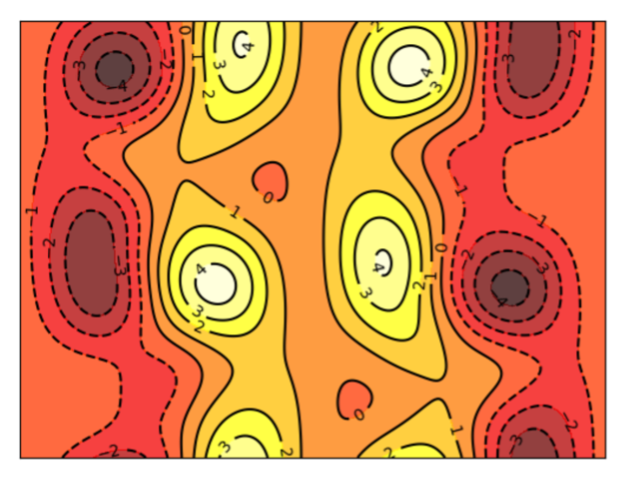
\includegraphics[width=0.8\linewidth]{images/Eijnden2018-heatmap-3dspin.png}
  \caption{ caption}
  \label{fig: description}
\end{subfigure}%
\begin{subfigure}{0.5\textwidth}
  \centering
  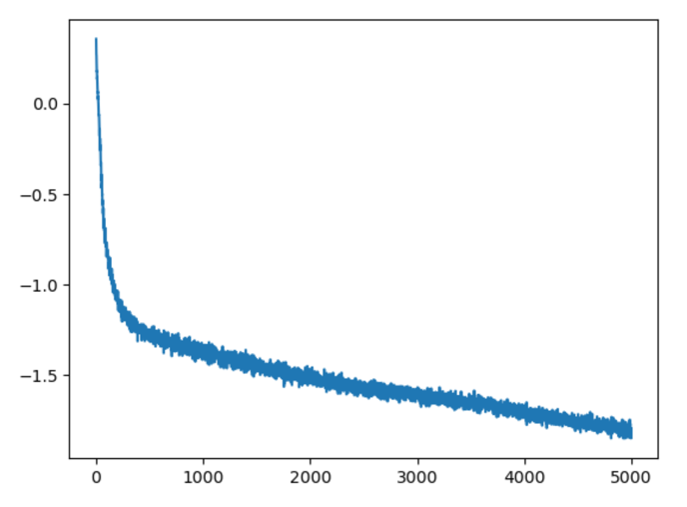
\includegraphics[width=0.8\linewidth]{images/Eijnden2018-loss.png}
  \caption{ caption}
  \label{fig:  description}
\end{subfigure}
\caption{Left panel: Comparison between the level sets of the original
  function $f$ in~\eqref{eq:psin} (black dotted curves) and its approximation
  by the neural network in~\eqref{eq:119} with $n= 128$ and $d=5$ in
  the slice defined by~\eqref{eq:slice}. Also shown are the projection
  in the slice of the particle position. Right panel: empirical loss in
  ~\eqref{eq:lossempirical} vs $n$ at the end of the calculation. The
  stars show the empirical loss for 10 independent
  realizations of the coefficients $a_{p,q,r}$ in~\eqref{eq:psin}.  }
\label{fig:  label}
\end{figure}




\subsection{Learning with Gaussian kernels}
\label{sec:gauss}

•	 Upon completing a preliminary reading of the \cite{Mei_2018} paper, my supervisor suggested that I look at the Vanden Eijnden et al paper \cite{Rotskoff_2022}, in particular the example with radially symmetric functions? 

•	Implemented gaussian kernel-approximation using SGD to 3-spin model, vanilla version and implemented an algorithm where no new sampling was necessary due to the network parameters and inputs having the same constraint.
•	
\subsection{Week 8-10}

I have implemented second-order methods, namely, Nesterov accelerated gradient descent and ‘Discretized mean field SGLD with homogenization’ as conceived in your paper entitled ‘The sharp, the flat and the shallow: Can weakly interacting agents learn to escape bad minima?’. I also came across a paper entitled ‘ACCELERATING SGD WITH MOMENTUM FOR OVER-PARAMETERIZED LEARNING’ by Liu and Belkin, where the authors claim that Nesterov SGD with any parameter selection does not in general provide acceleration over ordinary SGD’. There the authors come up with a modified algorithm which they call ‘Momentum-added stochastic solver (MaSS)’. I have made the following observations:
 
•	For the Isotropic Gaussian learning problem in the 2018 paper by Mei et al.
o	Nesterov-accelerated GD beats plain SGD, as expected
 
 
•	Anisotropic Gaussian learning problem in the 2018 paper by Mei et al.
o	Here Nesterov accelerated SGD performs the best, outperforming plain SGD, and while in the beginning, the MF-HomSGLD matches the performance of plain SGD, it seems to get stuck for larger iterations. 
 


\begin{figure}\centering
\subfloat[legend]{\label{a}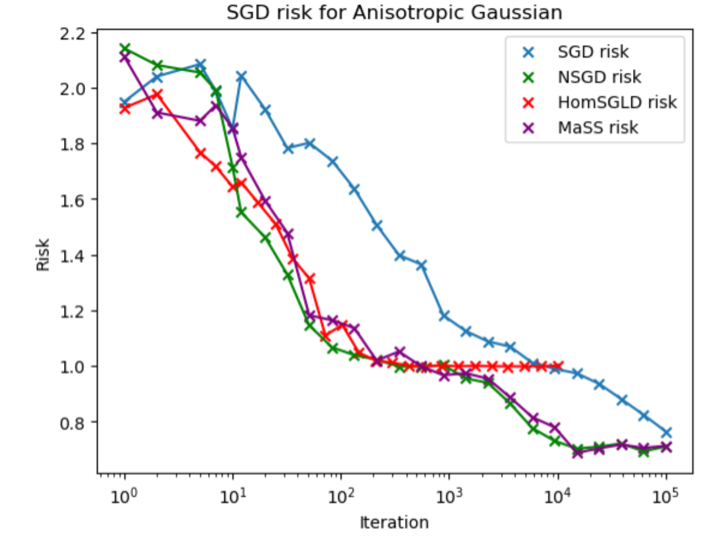
\includegraphics[width=.45\linewidth]{images/Nguyen2018-SGD-algos-risk-aniso-gauss.png}}\hfill
\subfloat[legend]{\label{b}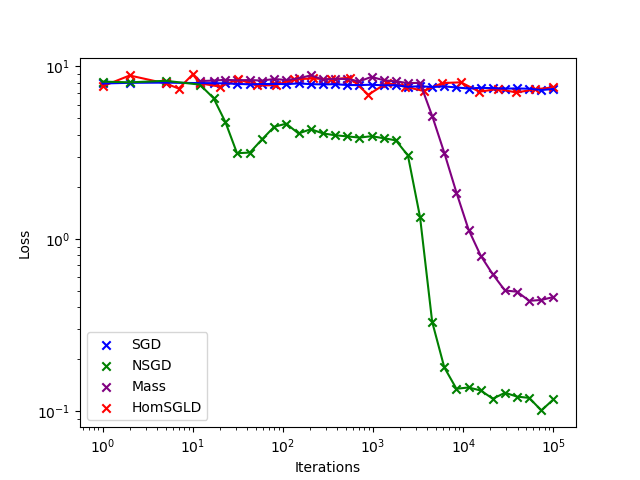
\includegraphics[width=.45\linewidth]{images/Nguyen2018-SGD-algos-risk-iso-gauss-non-mon.png}}\par 
\subfloat[legend]{\label{c}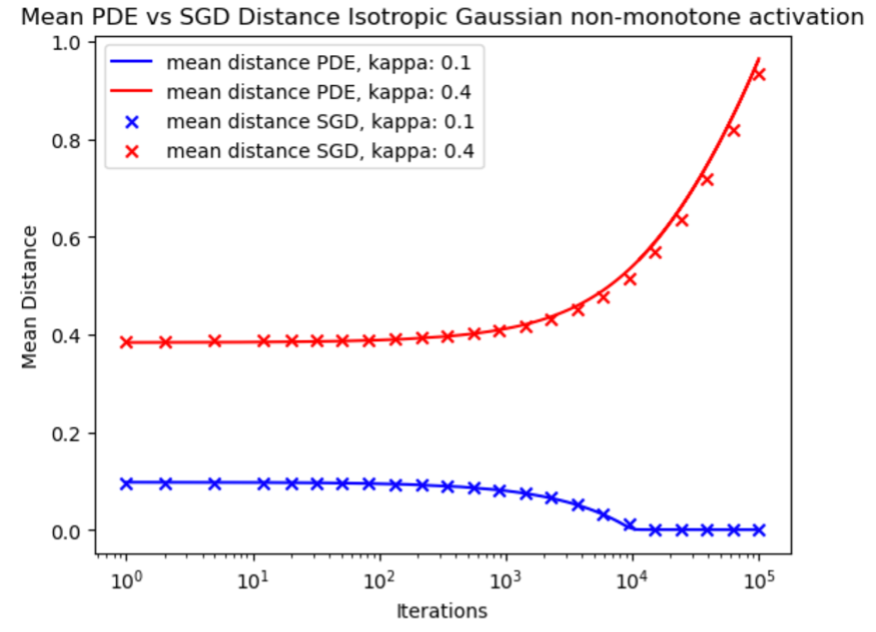
\includegraphics[width=.45\linewidth]{images/NGuyen2018-pde-sgd-iso-gauss-non-mon.png}}
\caption{my fig}
\label{fig}
\end{figure}


•	Isotropic Gaussian with non-monotone activation learning problem in the 2018 paper by Mei et al.
o	Here Nesterov accelerated and plain SGD were implemented
o	The non-monotone activation function in the neural network introduced some non-global minima where SGD seemed to get stuck, whereas Nesterov SGD seemed to avoid such ‘bad minima’ and attain monotonically decreasing losses characteristic of a global minimum. MF-HomSGLD seems to take longer to converge, maybe the hyper-parameters of the algorithm are not optimally tuned.
o	Here The MaSS algorithm seems to outperform the Nesterov accelerated sgd only in later iterations
 
 
•	3d-spin model considered in Vanden-Eijnden’s 2018 paper
o	In the deterministic gradient flow (with random initialization), the Nesterov accelerated loss (green) decreases  towards a minimum much faster than regular gradient descent (blue), as expected
 
o	In the stochastic gradient flow (with random initialization), the Nesterov accelerated loss (green) decreases  towards a minimum faster than regular gradient descent (blue), though the losses stay closer together
\begin{figure}[H]
  \centering
  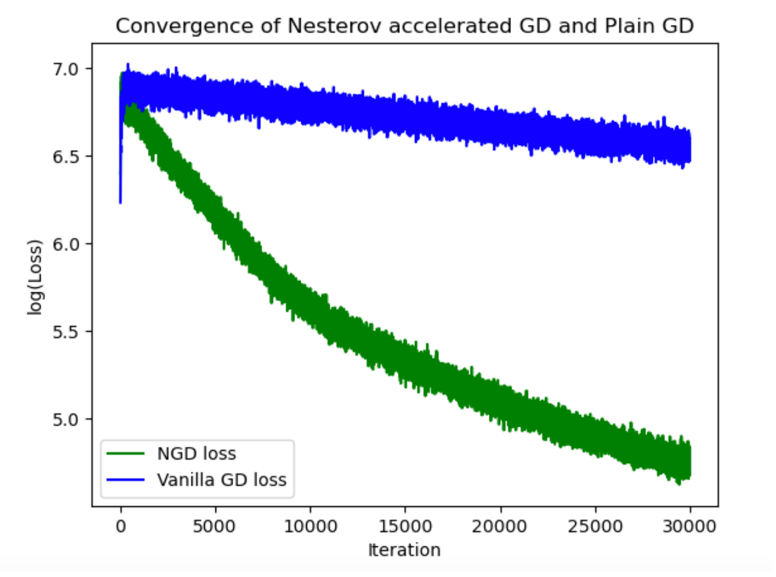
\includegraphics[width=0.8\textwidth]{images/Eijnden2018-SGD-algos-risk-3dspin.png}
  \caption{ caption}
  \label{fig: description}
\end{figure}%
 
•	Single-digit classification algorithm on the MNIST dataset
o	Nesterov acceleration beat plain SGD, but was beaten by MF-HomSGLD, which plateaued early but achieved a substantially smaller loss in the same amount of time
     \begin{figure}[H]
 \begin{subfigure}{0.5\textwidth}
   \centering
   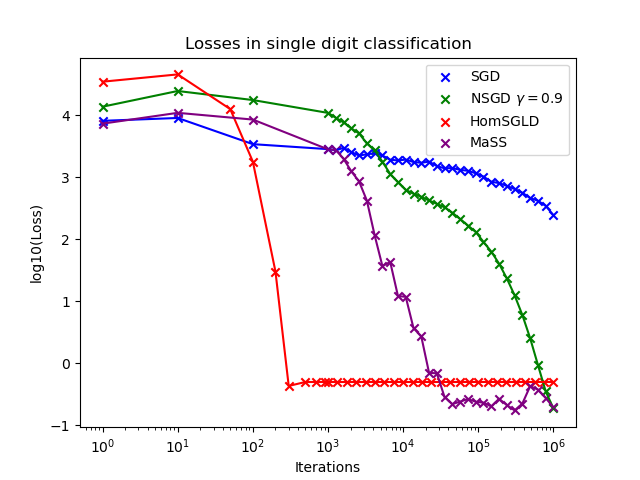
\includegraphics[width=0.8\linewidth]{images/Spiliopoulos2019-SGD-algos-single-digit classification.png}
   \caption{ caption}
   \label{fig: description}
 \end{subfigure}%
 \begin{subfigure}{0.5\textwidth}
   \centering
   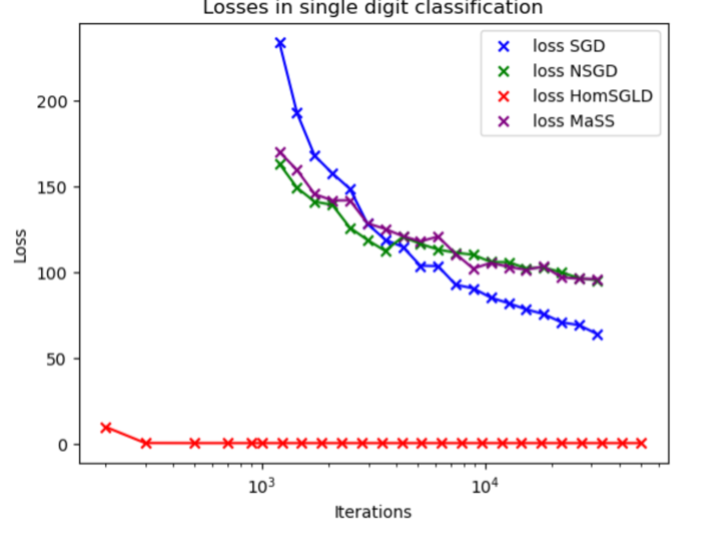
\includegraphics[width=0.8\linewidth]{images/Spiliopoulos2019-SGD-algos-single-digit-late-time.png}
   \caption{ caption}
   \label{fig:  description}
 \end{subfigure}
 \caption{ caption}
 \label{fig:  label}
 \end{figure} 


 \begin{figure}[H]\centering
\subfloat[legend]{\label{a}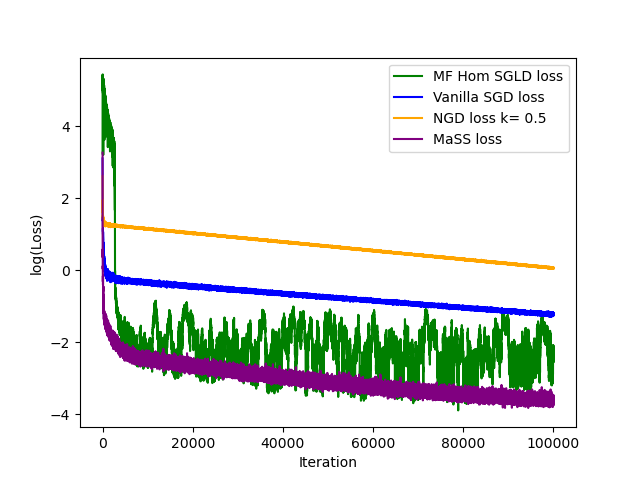
\includegraphics[width=.45\linewidth]{images/3d-spin-model-neural-net-loss-d=3.png}}\hfill
\subfloat[legend]{\label{b}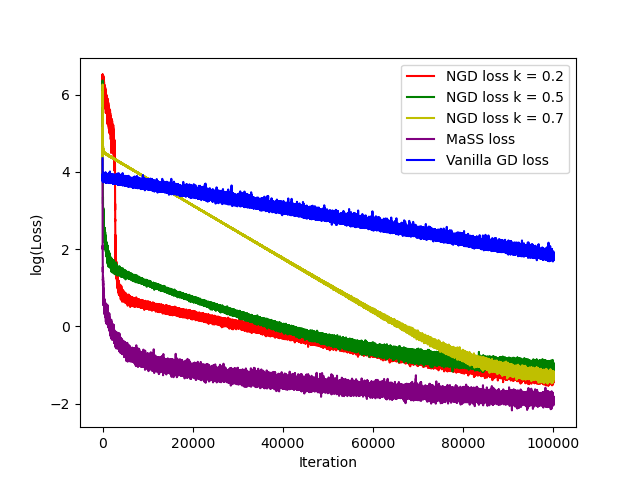
\includegraphics[width=.45\linewidth]{images/3d-spin-model-neural-net-loss-d=4.png}}\par 
\subfloat[legend]{\label{c}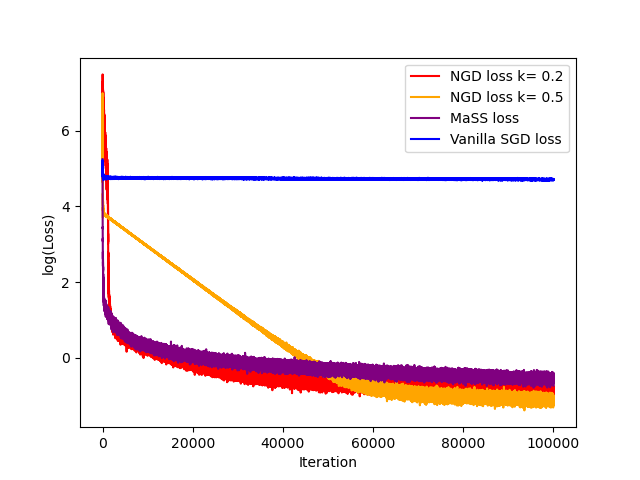
\includegraphics[width=.45\linewidth]{images/3d-spin-model-neural-net-loss-d=5.png}}
\caption{my fig}
\label{fig}
\end{figure}

\begin{figure}[H]\centering
\subfloat[legend]{\label{a}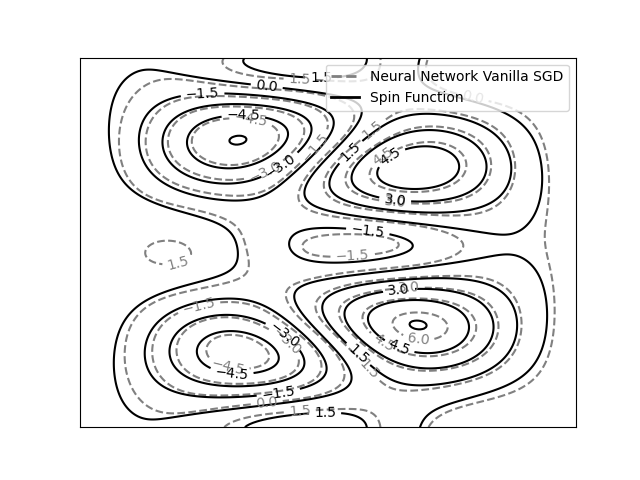
\includegraphics[width=.5\linewidth]{images/3d-spin-model-neural-net-plot-d=3.png}}\hfill
\subfloat[legend]{\label{b}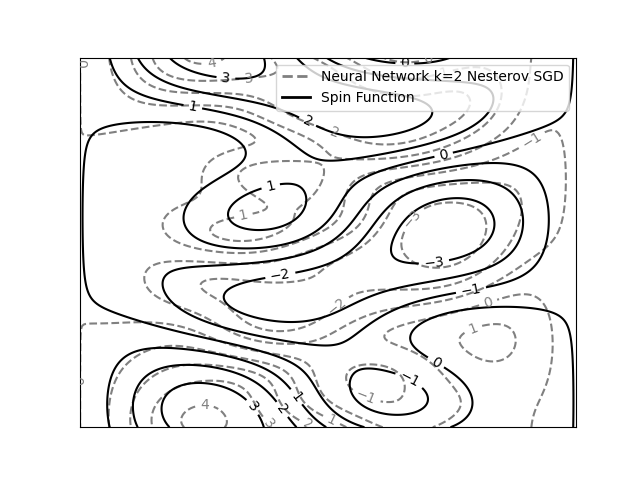
\includegraphics[width=.5\linewidth]{images/3d-spin-model-neural-net-plot-d=4.png}}\par 
\subfloat[legend]{\label{c}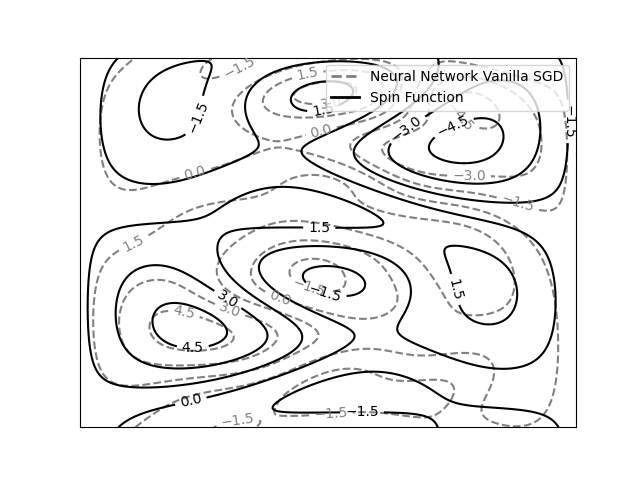
\includegraphics[width=.5\linewidth]{images/3d-spin-model-neural-net-plot-d=5.png}}
\caption{my fig}
\label{fig}
\end{figure}

Some general observations: 
•	For Nesterov accelerated descent:
o	In the deterministic case, as showcased by the 3d-spin model, Nesterov clearly beats plain GD;  this is to be expected.
o	This acceleration is harder to see in the stochastic setting. Nesterov-accelerated SGD seems on all occasions to perform better than plain SGD, but in some cases marginally so.
o	The more noteworthy observation is that it gets ‘unstuck’ at the ‘bad’ minimum in the non-monotone activation case.
•	The MF-HomSGLD algorithm:
o	I chose to implement this algorithm because it corresponds to a discretisation of a gradient flow with respect to a regularized potential.
o	MF-HomSGLD matches the performance of plain SGD, but it seems to get stuck for larger iterations and plateaus. However in the MNIST one-digit classification, the algorithm attains a substantially smaller loss, about two orders of magnitude less than the other algorithms, but it suffers from plateauing early again.
•	The MaSS algorithm: 
o	In most cases, despite claims in the paper by Liu and Belkin of exponential convergence (assuming certain regularity restraints on the loss which may be optimistic in my case), the performance at least matches Nesterov SGD, since it is a perturbation thereof. However, in the non-monotone activation function case, it beats all algorithms in later iterations and descends the fastest in loss.



\newpage
\bibliographystyle{plain}
\bibliography{references}

\end{document}
